%%%%%%%%%%%%%%%%%%%%%%%%%%%%%%%%%%%%%%%%%
%  My documentation report
%  Objetive: Explain what I did and how, so someone can continue with the investigation
%
% Important note:
% Chapter heading images should have a 2:1 width:height ratio,
% e.g. 920px width and 460px height.
%
%%%%%%%%%%%%%%%%%%%%%%%%%%%%%%%%%%%%%%%%%

%----------------------------------------------------------------------------------------
%	PACKAGES AND OTHER DOCUMENT CONFIGURATIONS
%----------------------------------------------------------------------------------------

\documentclass[11pt,fleqn]{book} % Default font size and left-justified equations

\usepackage[top=3cm,bottom=3cm,left=3.2cm,right=3.2cm,headsep=10pt,letterpaper]{geometry} % Page margins

\usepackage{xcolor} % Required for specifying colors by name
\definecolor{ocre}{RGB}{52,177,201} % Define the orange color used for highlighting throughout the book

% Font Settings
\usepackage{avant} % Use the Avantgarde font for headings
%\usepackage{times} % Use the Times font for headings
\usepackage{mathptmx} % Use the Adobe Times Roman as the default text font together with math symbols from the Sym­bol, Chancery and Com­puter Modern fonts

\usepackage{microtype} % Slightly tweak font spacing for aesthetics
\usepackage[utf8]{inputenc} % Required for including letters with accents
\usepackage[T1]{fontenc} % Use 8-bit encoding that has 256 glyphs

% Bibliography
\usepackage[style=alphabetic,sorting=nyt,sortcites=true,autopunct=true,babel=hyphen,hyperref=true,abbreviate=false,backref=true,backend=biber]{biblatex}
\addbibresource{bibliography.bib} % BibTeX bibliography file
\defbibheading{bibempty}{}

%----------------------------------------------------------------------------------------
%	VARIOUS REQUIRED PACKAGES
%----------------------------------------------------------------------------------------

\usepackage{titlesec} % Allows customization of titles

\usepackage{graphicx} % Required for including pictures
\graphicspath{{Pictures/}} % Specifies the directory where pictures are stored

\usepackage{lipsum} % Inserts dummy text

\usepackage{tikz} % Required for drawing custom shapes

\usepackage[english]{babel} % English language/hyphenation

\usepackage{enumitem} % Customize lists
\setlist{nolistsep} % Reduce spacing between bullet points and numbered lists

\usepackage{booktabs} % Required for nicer horizontal rules in tables

\usepackage{eso-pic} % Required for specifying an image background in the title page

%----------------------------------------------------------------------------------------
%	MAIN TABLE OF CONTENTS
%----------------------------------------------------------------------------------------

\usepackage{titletoc} % Required for manipulating the table of contents

\contentsmargin{0cm} % Removes the default margin
% Chapter text styling
\titlecontents{chapter}[1.25cm] % Indentation
{\addvspace{15pt}\large\sffamily\bfseries} % Spacing and font options for chapters
{\color{ocre!60}\contentslabel[\Large\thecontentslabel]{1.25cm}\color{ocre}} % Chapter number
{}  
{\color{ocre!60}\normalsize\sffamily\bfseries\;\titlerule*[.5pc]{.}\;\thecontentspage} % Page number
% Section text styling
\titlecontents{section}[1.25cm] % Indentation
{\addvspace{5pt}\sffamily\bfseries} % Spacing and font options for sections
{\contentslabel[\thecontentslabel]{1.25cm}} % Section number
{}
{\color{black}\sffamily\;\titlerule*[.5pc]{.}\;\thecontentspage} % Page number
[]
% Subsection text styling
\titlecontents{subsection}[1.25cm] % Indentation
{\addvspace{1pt}\sffamily\small} % Spacing and font options for subsections
{\contentslabel[\thecontentslabel]{1.25cm}} % Subsection number
{}
{\sffamily\;\titlerule*[.5pc]{.}\;\thecontentspage} % Page number
[] 

%----------------------------------------------------------------------------------------
%	MINI TABLE OF CONTENTS IN CHAPTER HEADS
%----------------------------------------------------------------------------------------

% Section text styling
\titlecontents{lsection}[0em] % Indendating
{\footnotesize\sffamily} % Font settings
{}
{}
{}

% Subsection text styling
\titlecontents{lsubsection}[.5em] % Indentation
{\normalfont\footnotesize\sffamily} % Font settings
{}
{}
{}
 
%----------------------------------------------------------------------------------------
%	PAGE HEADERS
%----------------------------------------------------------------------------------------

\usepackage{fancyhdr} % Required for header and footer configuration

\pagestyle{fancy}
\renewcommand{\chaptermark}[1]{\markboth{\sffamily\normalsize\bfseries\chaptername\ \thechapter.\ #1}{}} % Chapter text font settings
\renewcommand{\sectionmark}[1]{\markright{\sffamily\normalsize\thesection\hspace{5pt}#1}{}} % Section text font settings
\fancyhf{} \fancyhead[LE,RO]{\sffamily\normalsize\thepage} % Font setting for the page number in the header
\fancyhead[LO]{\rightmark} % Print the nearest section name on the left side of odd pages
\fancyhead[RE]{\leftmark} % Print the current chapter name on the right side of even pages
\renewcommand{\headrulewidth}{0.5pt} % Width of the rule under the header
\addtolength{\headheight}{2.5pt} % Increase the spacing around the header slightly
\renewcommand{\footrulewidth}{0pt} % Removes the rule in the footer
\fancypagestyle{plain}{\fancyhead{}\renewcommand{\headrulewidth}{0pt}} % Style for when a plain pagestyle is specified

% Removes the header from odd empty pages at the end of chapters
\makeatletter
\renewcommand{\cleardoublepage}{
\clearpage\ifodd\c@page\else
\hbox{}
\vspace*{\fill}
\thispagestyle{empty}
\newpage
\fi}

%----------------------------------------------------------------------------------------
%	THEOREM STYLES
%----------------------------------------------------------------------------------------

\usepackage{amsmath,amsfonts,amssymb,amsthm} % For math equations, theorems, symbols, etc

\newcommand{\intoo}[2]{\mathopen{]}#1\,;#2\mathclose{[}}
\newcommand{\ud}{\mathop{\mathrm{{}d}}\mathopen{}}
\newcommand{\intff}[2]{\mathopen{[}#1\,;#2\mathclose{]}}
\newtheorem{notation}{Notation}[chapter]

%%%%%%%%%%%%%%%%%%%%%%%%%%%%%%%%%%%%%%%%%%%%%%%%%%%%%%%%%%%%%%%%%%%%%%%%%%%
%%%%%%%%%%%%%%%%%%%% dedicated to boxed/framed environements %%%%%%%%%%%%%%
%%%%%%%%%%%%%%%%%%%%%%%%%%%%%%%%%%%%%%%%%%%%%%%%%%%%%%%%%%%%%%%%%%%%%%%%%%%
\newtheoremstyle{ocrenumbox}% % Theorem style name
{0pt}% Space above
{0pt}% Space below
{\normalfont}% % Body font
{}% Indent amount
{\small\bf\sffamily\color{ocre}}% % Theorem head font
{\;}% Punctuation after theorem head
{0.25em}% Space after theorem head
{\small\sffamily\color{ocre}\thmname{#1}\nobreakspace\thmnumber{\@ifnotempty{#1}{}\@upn{#2}}% Theorem text (e.g. Theorem 2.1)
\thmnote{\nobreakspace\the\thm@notefont\sffamily\bfseries\color{black}---\nobreakspace#3.}} % Optional theorem note
\renewcommand{\qedsymbol}{$\blacksquare$}% Optional qed square

\newtheoremstyle{blacknumex}% Theorem style name
{5pt}% Space above
{5pt}% Space below
{\normalfont}% Body font
{} % Indent amount
{\small\bf\sffamily}% Theorem head font
{\;}% Punctuation after theorem head
{0.25em}% Space after theorem head
{\small\sffamily{\tiny\ensuremath{\blacksquare}}\nobreakspace\thmname{#1}\nobreakspace\thmnumber{\@ifnotempty{#1}{}\@upn{#2}}% Theorem text (e.g. Theorem 2.1)
\thmnote{\nobreakspace\the\thm@notefont\sffamily\bfseries---\nobreakspace#3.}}% Optional theorem note

\newtheoremstyle{blacknumbox} % Theorem style name
{0pt}% Space above
{0pt}% Space below
{\normalfont}% Body font
{}% Indent amount
{\small\bf\sffamily}% Theorem head font
{\;}% Punctuation after theorem head
{0.25em}% Space after theorem head
{\small\sffamily\thmname{#1}\nobreakspace\thmnumber{\@ifnotempty{#1}{}\@upn{#2}}% Theorem text (e.g. Theorem 2.1)
\thmnote{\nobreakspace\the\thm@notefont\sffamily\bfseries---\nobreakspace#3.}}% Optional theorem note

%%%%%%%%%%%%%%%%%%%%%%%%%%%%%%%%%%%%%%%%%%%%%%%%%%%%%%%%%%%%%%%%%%%%%%%%%%%
%%%%%%%%%%%%% dedicated to non-boxed/non-framed environements %%%%%%%%%%%%%
%%%%%%%%%%%%%%%%%%%%%%%%%%%%%%%%%%%%%%%%%%%%%%%%%%%%%%%%%%%%%%%%%%%%%%%%%%%
\newtheoremstyle{ocrenum}% % Theorem style name
{5pt}% Space above
{5pt}% Space below
{\normalfont}% % Body font
{}% Indent amount
{\small\bf\sffamily\color{ocre}}% % Theorem head font
{\;}% Punctuation after theorem head
{0.25em}% Space after theorem head
{\small\sffamily\color{ocre}\thmname{#1}\nobreakspace\thmnumber{\@ifnotempty{#1}{}\@upn{#2}}% Theorem text (e.g. Theorem 2.1)
\thmnote{\nobreakspace\the\thm@notefont\sffamily\bfseries\color{black}---\nobreakspace#3.}} % Optional theorem note
\renewcommand{\qedsymbol}{$\blacksquare$}% Optional qed square
\makeatother

% Defines the theorem text style for each type of theorem to one of the three styles above
\newcounter{dummy} 
\numberwithin{dummy}{section}
\theoremstyle{ocrenumbox}
\newtheorem{theoremeT}[dummy]{Theorem}
\newtheorem{problem}{Problem}[chapter]
\newtheorem{exerciseT}{Exercise}[chapter]
\theoremstyle{blacknumex}
\newtheorem{exampleT}{Example}[chapter]
\theoremstyle{blacknumbox}
\newtheorem{vocabulary}{Vocabulary}[chapter]
\newtheorem{definitionT}{Definition}[section]
\newtheorem{corollaryT}[dummy]{Corollary}
\theoremstyle{ocrenum}
\newtheorem{proposition}[dummy]{Proposition}

%----------------------------------------------------------------------------------------
%	DEFINITION OF COLORED BOXES
%----------------------------------------------------------------------------------------

\RequirePackage[framemethod=default]{mdframed} % Required for creating the theorem, definition, exercise and corollary boxes

% Theorem box
\newmdenv[skipabove=7pt,
skipbelow=7pt,
backgroundcolor=black!5,
linecolor=ocre,
innerleftmargin=5pt,
innerrightmargin=5pt,
innertopmargin=5pt,
leftmargin=0cm,
rightmargin=0cm,
innerbottommargin=5pt]{tBox}

% Exercise box	  
\newmdenv[skipabove=7pt,
skipbelow=7pt,
rightline=false,
leftline=true,
topline=false,
bottomline=false,
backgroundcolor=ocre!10,
linecolor=ocre,
innerleftmargin=5pt,
innerrightmargin=5pt,
innertopmargin=5pt,
innerbottommargin=5pt,
leftmargin=0cm,
rightmargin=0cm,
linewidth=4pt]{eBox}	

% Definition box
\newmdenv[skipabove=7pt,
skipbelow=7pt,
rightline=false,
leftline=true,
topline=false,
bottomline=false,
linecolor=ocre,
innerleftmargin=5pt,
innerrightmargin=5pt,
innertopmargin=0pt,
leftmargin=0cm,
rightmargin=0cm,
linewidth=4pt,
innerbottommargin=0pt]{dBox}	

% Corollary box
\newmdenv[skipabove=7pt,
skipbelow=7pt,
rightline=false,
leftline=true,
topline=false,
bottomline=false,
linecolor=gray,
backgroundcolor=black!5,
innerleftmargin=5pt,
innerrightmargin=5pt,
innertopmargin=5pt,
leftmargin=0cm,
rightmargin=0cm,
linewidth=4pt,
innerbottommargin=5pt]{cBox}

% Creates an environment for each type of theorem and assigns it a theorem text style from the "Theorem Styles" section above and a colored box from above
\newenvironment{theorem}{\begin{tBox}\begin{theoremeT}}{\end{theoremeT}\end{tBox}}
\newenvironment{exercise}{\begin{eBox}\begin{exerciseT}}{\hfill{\color{ocre}\tiny\ensuremath{\blacksquare}}\end{exerciseT}\end{eBox}}				  
\newenvironment{definition}{\begin{dBox}\begin{definitionT}}{\end{definitionT}\end{dBox}}	
\newenvironment{example}{\begin{exampleT}}{\hfill{\tiny\ensuremath{\blacksquare}}\end{exampleT}}		
\newenvironment{corollary}{\begin{cBox}\begin{corollaryT}}{\end{corollaryT}\end{cBox}}	

%----------------------------------------------------------------------------------------
%	REMARK ENVIRONMENT
%----------------------------------------------------------------------------------------

\newenvironment{remark}{\par\vspace{10pt}\small % Vertical white space above the remark and smaller font size
\begin{list}{}{
\leftmargin=35pt % Indentation on the left
\rightmargin=25pt}\item\ignorespaces % Indentation on the right
\makebox[-2.5pt]{\begin{tikzpicture}[overlay]
\node[draw=ocre!60,line width=1pt,circle,fill=ocre!25,font=\sffamily\bfseries,inner sep=2pt,outer sep=0pt] at (-15pt,0pt){\textcolor{ocre}{R}};\end{tikzpicture}} % Orange R in a circle
\advance\baselineskip -1pt}{\end{list}\vskip5pt} % Tighter line spacing and white space after remark

%----------------------------------------------------------------------------------------
%	SECTION NUMBERING IN THE MARGIN
%----------------------------------------------------------------------------------------

\makeatletter
\renewcommand{\@seccntformat}[1]{\llap{\textcolor{ocre}{\csname the#1\endcsname}\hspace{1em}}}                    
\renewcommand{\section}{\@startsection{section}{1}{\z@}
{-4ex \@plus -1ex \@minus -.4ex}
{1ex \@plus.2ex }
{\normalfont\large\sffamily\bfseries}}
\renewcommand{\subsection}{\@startsection {subsection}{2}{\z@}
{-3ex \@plus -0.1ex \@minus -.4ex}
{0.5ex \@plus.2ex }
{\normalfont\sffamily\bfseries}}
\renewcommand{\subsubsection}{\@startsection {subsubsection}{3}{\z@}
{-2ex \@plus -0.1ex \@minus -.2ex}
{.2ex \@plus.2ex }
{\normalfont\small\sffamily\bfseries}}                        
\renewcommand\paragraph{\@startsection{paragraph}{4}{\z@}
{-2ex \@plus-.2ex \@minus .2ex}
{.1ex}
{\normalfont\small\sffamily\bfseries}}

%----------------------------------------------------------------------------------------
%	HYPERLINKS IN THE DOCUMENTS
%----------------------------------------------------------------------------------------

% For an unclear reason, the package should be loaded now and not later
\usepackage{hyperref}
%\hypersetup{hidelinks,backref=true,pagebackref=true,hyperindex=true,colorlinks=false,breaklinks=true,urlcolor= ocre,bookmarks=true,bookmarksopen=false,pdftitle={Title},pdfauthor={Author}}

%----------------------------------------------------------------------------------------
%	CHAPTER HEADINGS
%----------------------------------------------------------------------------------------

% The set-up below should be (sadly) manually adapted to the overall margin page septup controlled by the geometry package loaded in the main.tex document.
%It is possible to implement below the dimensions used in the goemetry package (top,bottom,left,right)... TO BE DONE

\newcommand{\thechapterimage}{}
\newcommand{\chapterimage}[1]{\renewcommand{\thechapterimage}{#1}}

% Numbered chapters with mini tableofcontents
\def\thechapter{\arabic{chapter}}
\def\@makechapterhead#1{
\thispagestyle{empty}
{\centering \normalfont\sffamily
\ifnum \c@secnumdepth >\m@ne
\if@mainmatter
\startcontents
\begin{tikzpicture}[remember picture,overlay]
\node at (current page.north west)
{\begin{tikzpicture}[remember picture,overlay]
\node[anchor=north west,inner sep=0pt] at (0,0) {\includegraphics[width=\paperwidth]{\thechapterimage}};
%%%%%%%%%%%%%%%%%%%%%%%%%%%%%%%%%%%%%%%%%%%%%%%%%%%%%%%%%%%%%%%%%%%%%%%%%%%%%%%%%%%%%
% Commenting the 3 lines below removes the small contents box in the chapter heading
%\fill[color=ocre!10!white,opacity=.6] (1cm,0) rectangle (8cm,-7cm);
%\node[anchor=north west] at (1.1cm,.35cm) {\parbox[t][8cm][t]{6.5cm}{\huge\bfseries\flushleft \printcontents{l}{1}{\setcounter{tocdepth}{2}}}};
\draw[anchor=west] (6cm,-6.5cm) node [rounded corners=20pt,fill=ocre!10!white,text opacity=1,draw=ocre,draw opacity=1,line width=1.5pt,fill opacity=.6,inner sep=12pt]{\huge\sffamily\bfseries\textcolor{black}{\thechapter. #1\strut\makebox[22cm]{}}};
%%%%%%%%%%%%%%%%%%%%%%%%%%%%%%%%%%%%%%%%%%%%%%%%%%%%%%%%%%%%%%%%%%%%%%%%%%%%%%%%%%%%%
\end{tikzpicture}};
\end{tikzpicture}}
\par\vspace*{200\p@}%Edited vertical spacing within TikZ picture to account for incorrect image Size -GY
\fi
\fi}

% Unnumbered chapters without mini tableofcontents (could be added though) 
\def\@makeschapterhead#1{
\thispagestyle{empty}
{\centering \normalfont\sffamily
\ifnum \c@secnumdepth >\m@ne
\if@mainmatter
\begin{tikzpicture}[remember picture,overlay]
\node at (current page.north west)
{\begin{tikzpicture}[remember picture,overlay]
\node[anchor=north west,inner sep=0pt] at (0,0) {\includegraphics[width=\paperwidth]{\thechapterimage}};
\draw[anchor=west] (6cm,-6.5cm) node [rounded corners=20pt,fill=ocre!10!white,fill opacity=.6,inner sep=12pt,text opacity=1,draw=ocre,draw opacity=1,line width=1.5pt]{\huge\sffamily\bfseries\textcolor{black}{#1\strut\makebox[22cm]{}}};
\end{tikzpicture}};
\end{tikzpicture}}
\par\vspace*{200\p@}%edited vertical spacing here as well to account for unnumbered chapters
\fi
\fi
}
\makeatother
 % Insert the commands.tex file which contains the majority of the structure behind the template

\begin{document}

%----------------------------------------------------------------------------------------
%	TITLE PAGE
%----------------------------------------------------------------------------------------

\begingroup
\thispagestyle{empty}
\AddToShipoutPicture*{\put(0,0){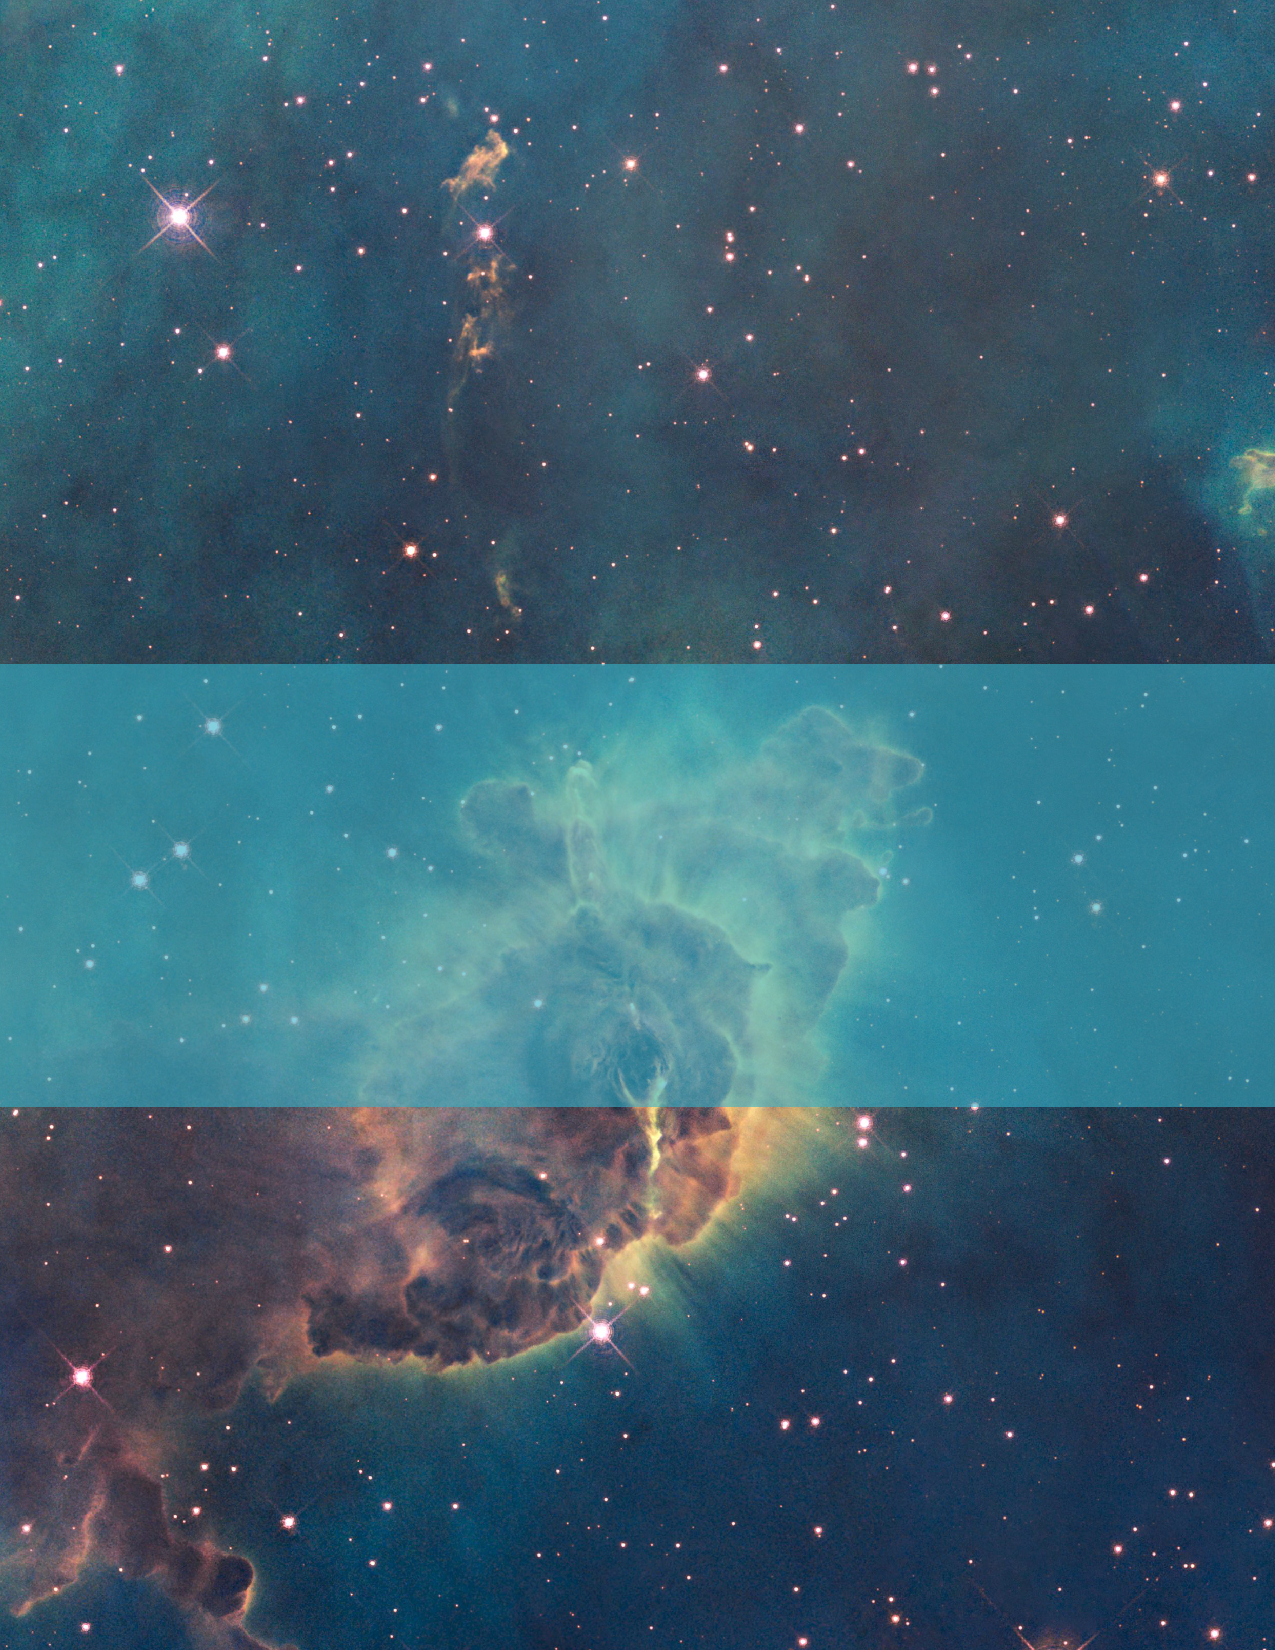
\includegraphics[scale=1.25]{esahubble}}} % Image background
%\AddToShipoutPicture*{\put(0,0){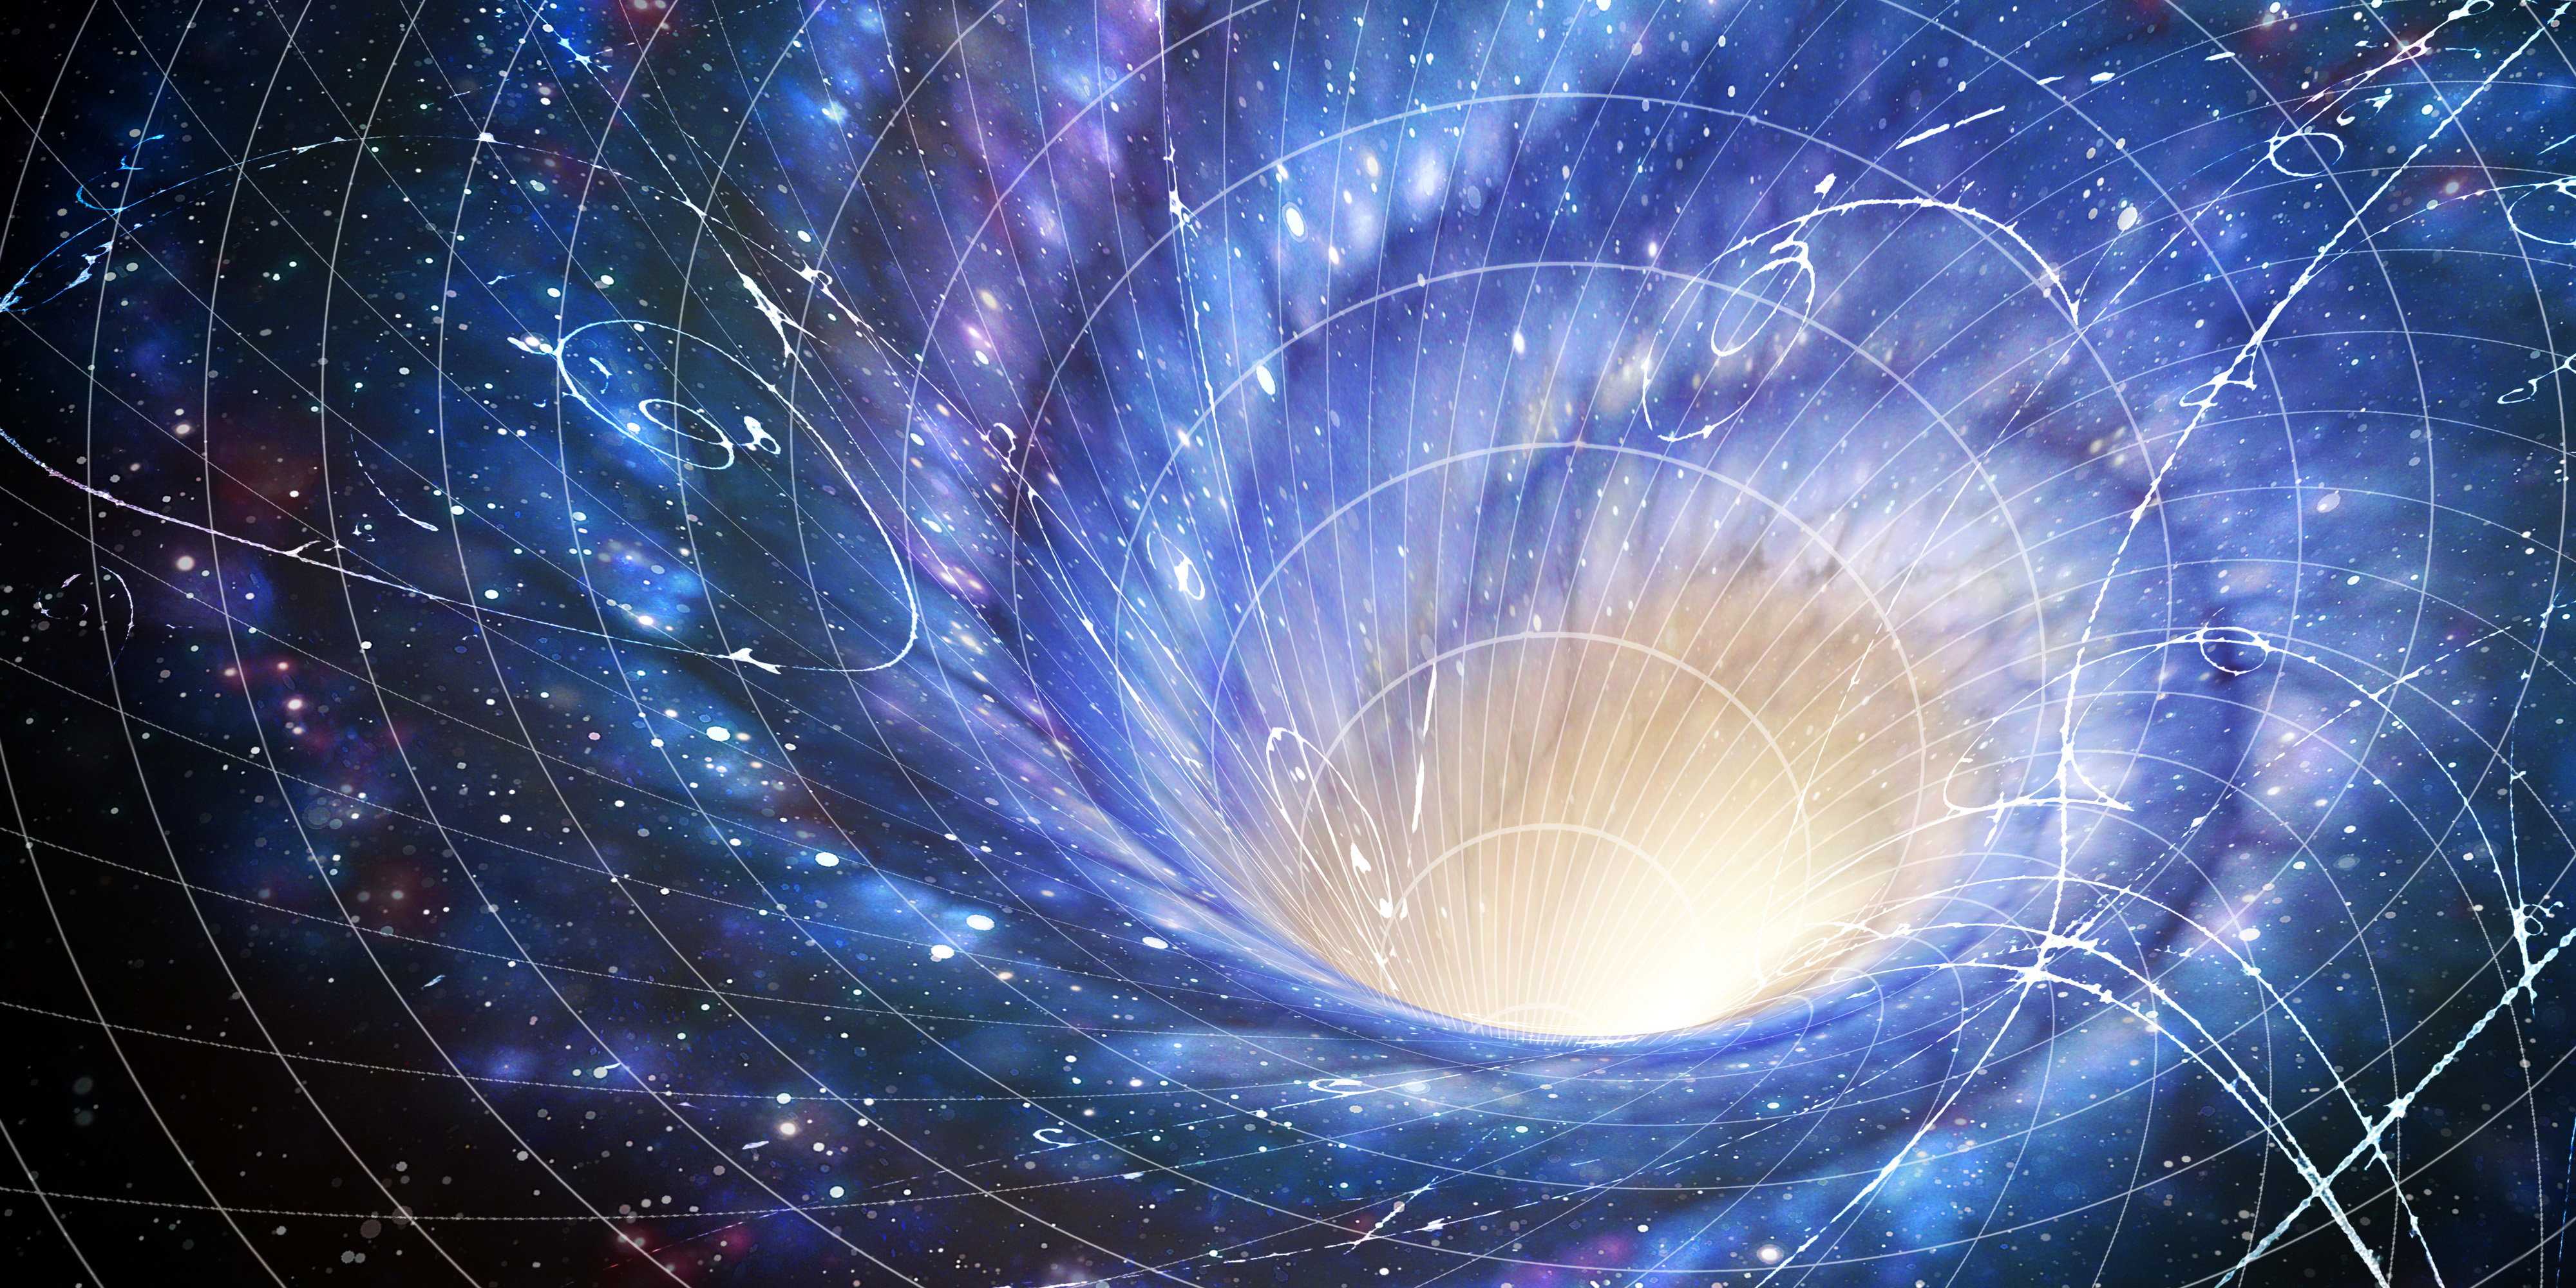
\includegraphics[scale=1.0]{galaxy_spacewarp.jpg}}}
\centering
\vspace*{5cm}
\par\normalfont\fontsize{35}{35}\sffamily\selectfont
\textbf{Case Studies using the R Programming Language}\\
{\LARGE }\par % Book title
\vspace*{1cm}
{\Large Katherine Bennett, Miguel delosReyes, Raymond Gao, Sophia Hurr, Hannah Gahagan, \\ Nikhil Miland, Mridu Nanda, Christa Parrish, Ishaan Rao, Grayson York,  \\ }\par % Author name
\endgroup

%----------------------------------------------------------------------------------------
%	COPYRIGHT PAGE
%----------------------------------------------------------------------------------------

\newpage
~\vfill
\thispagestyle{empty}

%\noindent Copyright \copyright\ 2014 Andrea Hidalgo\\ % Copyright notice

\noindent \textsc{Research in Computational Science}\\

\noindent \textsc{North Carolina School of Science and Mathematics, Durham, NC}\\ % URL

\noindent This case studies manual was prepared under the direction of Mr. Robert Gotwals, faculty mentor, The North Carolina School of Science and Mathematics, Durham NC.  \\ % License information

\noindent \textit{First release, November 2016} % Printing/edition date

%----------------------------------------------------------------------------------------
%	TABLE OF CONTENTS
%----------------------------------------------------------------------------------------

\chapterimage{galaxy_spacewarp.jpg} % Table of contents heading image

\pagestyle{empty} % No headers

\tableofcontents % Print the table of contents itself

%\cleardoublepage % Forces the first chapter to start on an odd page so it's on the right

\pagestyle{fancy} % Print headers again

%----------------------------------------------------------------------------------------
%	CHAPTER 1
%----------------------------------------------------------------------------------------

\chapterimage{galaxy_spacewarp.jpg} % Chapter heading image

\chapter{Introduction}

Gotwals will write an Intro. 

\subsection{References}\index{References}

\begin{remark}
For more information about the cosmological principle, review Chapter 1: Why Learn Astronomy?, page 10, from \textbf{21st Century Astronomy}, \textit{Hester | Smith | Blumenthal | Kay | Voss}, Third Edition, 2010.
\end{remark}

%This statement requires citation \cite{book_key}; this one is more specific \cite[122]{article_key}.


%----------------------------------------------------------------------------------------
%	CHAPTER 2
%----------------------------------------------------------------------------------------
\chapterimage{galaxy_spacewarp.jpg}

\chapter{Case Study 1:  xxxxxxxx}

\section{First ideas}\index{First ideas}
So, now here you have your first astronomy picture, \footnote{For example purposes the image selected is a picture of M83 through a Wide H-alpha and [N II] filter. } what do you see?, it is a monochrome image, with different levels of brightness, slightly big (8500 x 5000), it looks like a lot of stars making a spiral.
\begin{figure}[h]
    \centering
    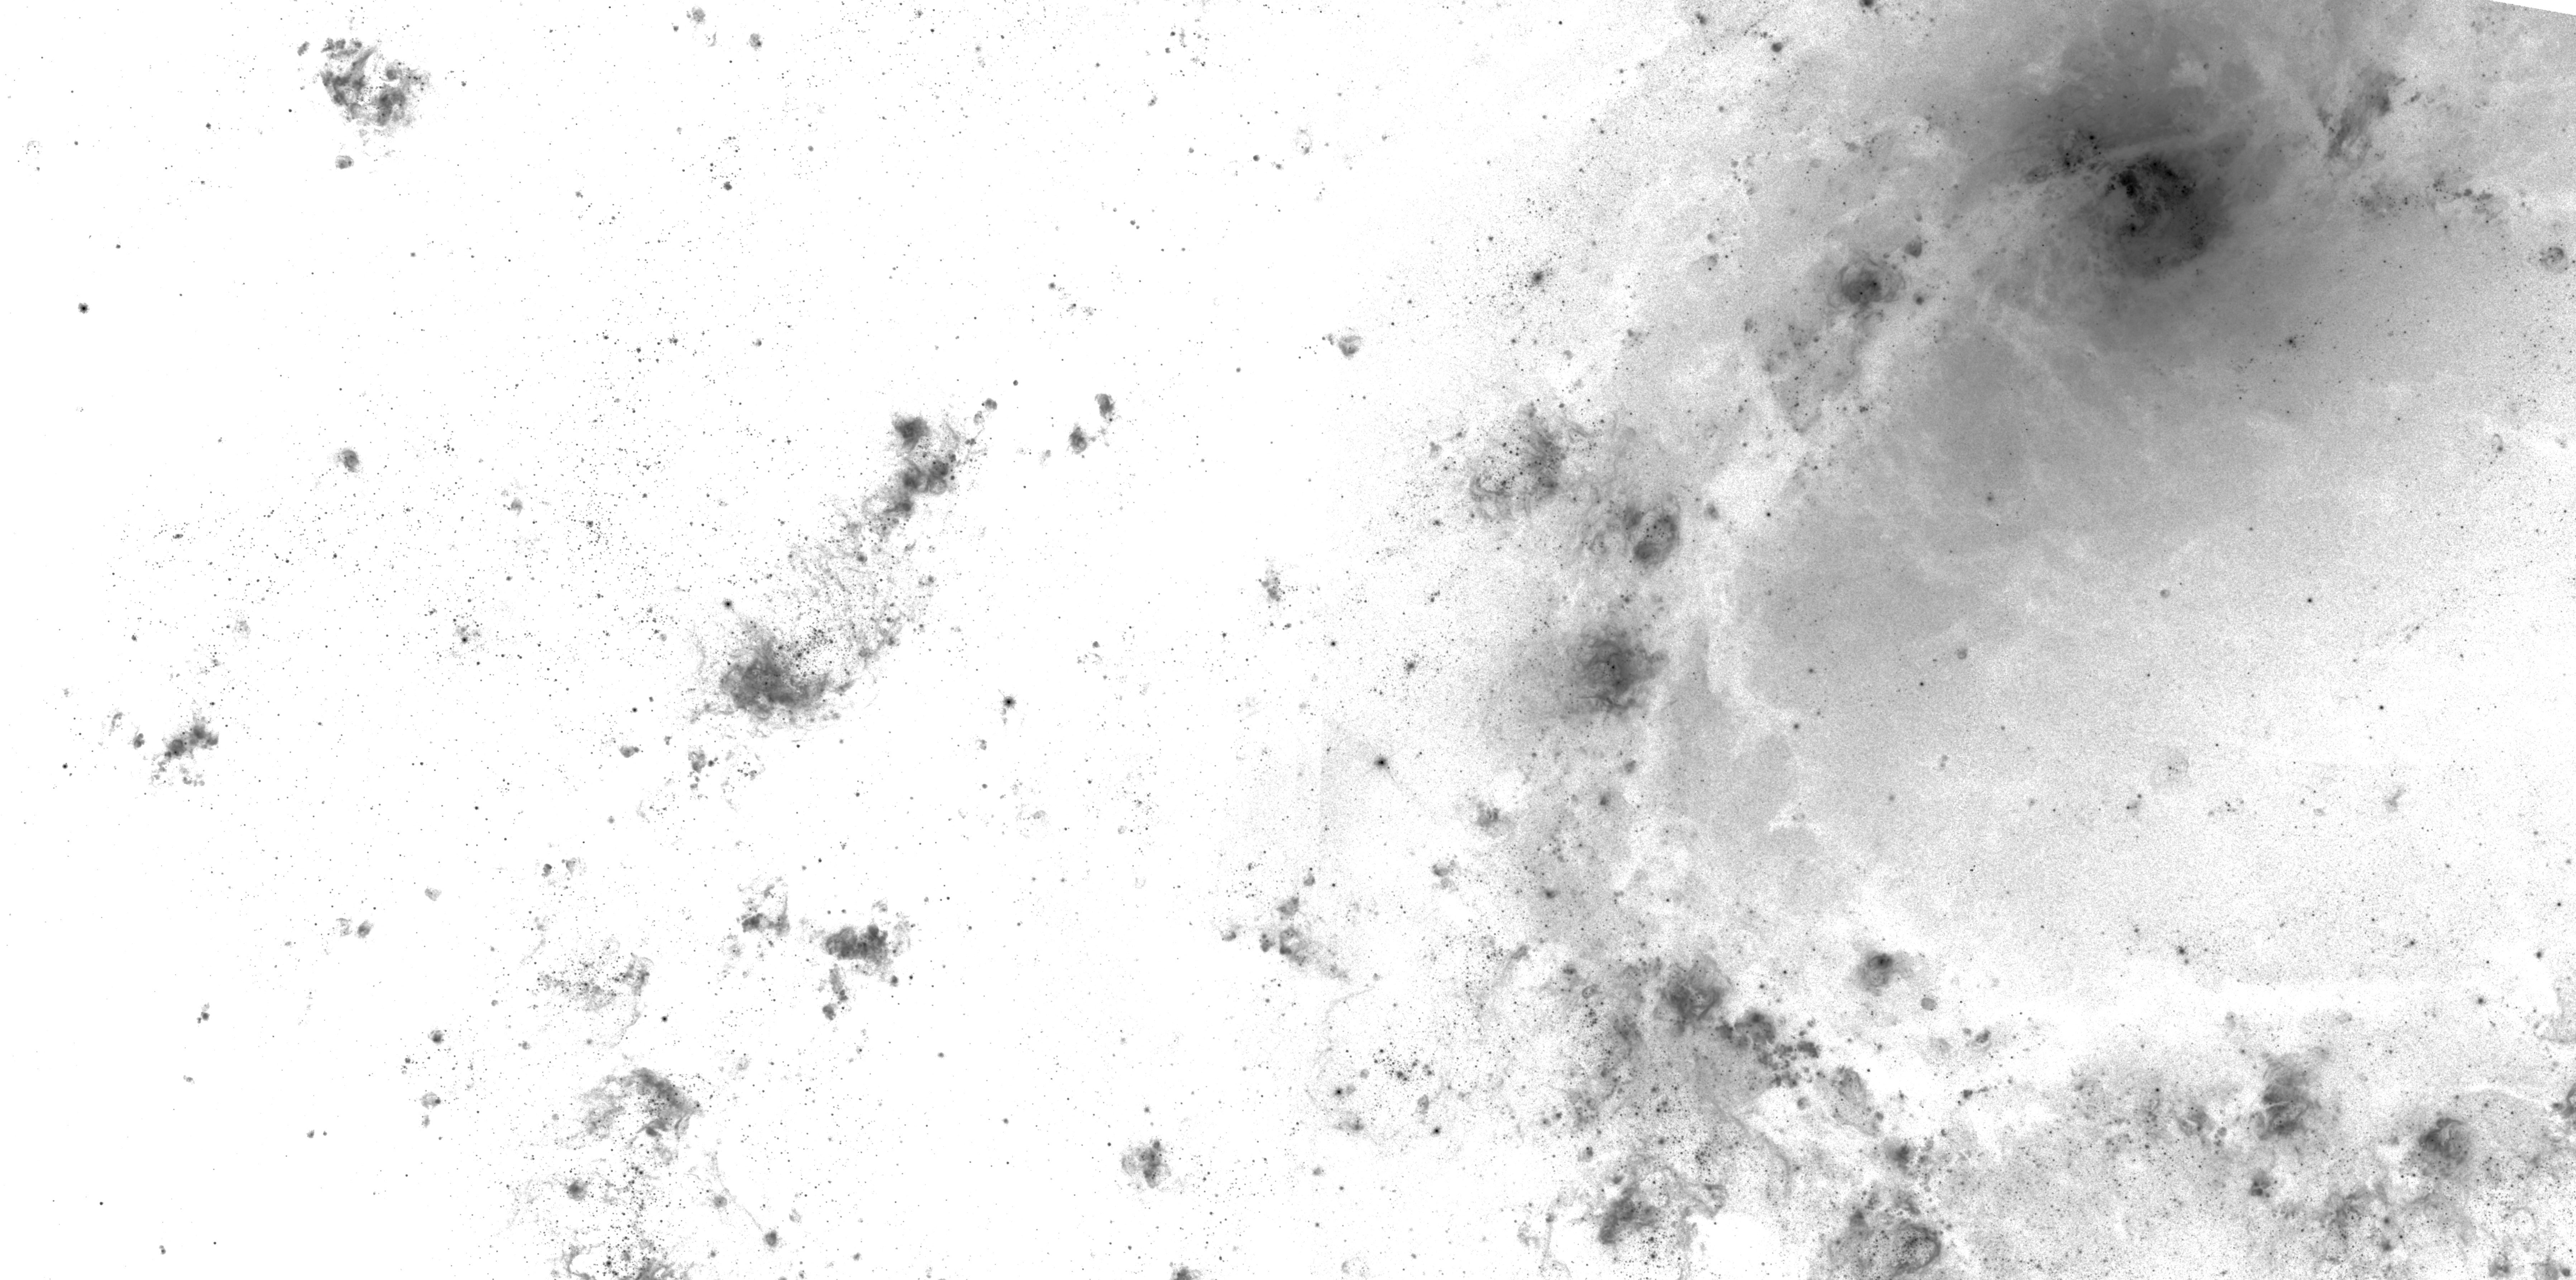
\includegraphics[width=0.77\textwidth]{ha-gray-conv-crp.jpg}
    \caption{Picuture of the M83 galaxy, image taken from the WFC3 ERS M83 Data Products, http://archive.stsci.edu/prepds/wfc3ers/m83datalist.html}
    \label{fig:awesome_image}
\end{figure}

How can we learn something about this image, quantize, get useful information? In the next subsections I will explain the first ideas.

\subsection{Superpixel segmentation}
The main concept of this is to cut an image into bigger neighborhood sections, so from an image that has $425x10^5$ pixels we can get maybe less than 500 superpixels, and then analyse separately those little sections and identify what kind of intersellar objects are they, look at image \ref{fig:super} it is a self-explanatory example of how a superpixel algorithm works.
\begin{figure}[h]
    \centering
    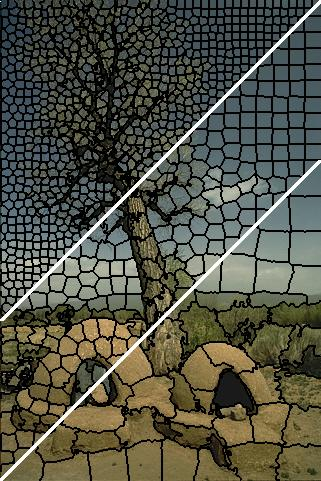
\includegraphics[width=0.37\textwidth]{combo.jpg}
    \caption{Example of a superpixel algorithm}
    \label{fig:super}
\end{figure}
There are many ways to do this and they vary according to color dimensions, methods and number of required superpixels and whether the algorithm is able to find borders and make pixel clasifications.

\begin{remark}
	You can find some example test I tested with Matlab and with Python in this webapage: \url{https://github.com/LaurethTeX/Clustering/blob/master/Methods.md}, also there is a huge amount of information on th internet about this but here are two pages you might find useful:
    \begin{itemize}
    	\item Superpixel: Empirical Studies and Applications \\ \url{http://ttic.uchicago.edu/~xren/research/superpixel/}
        \item Segmentation Algorithms in scikits-image \\ \url{http://peekaboo-vision.blogspot.ca/2012/09/segmentation-algorithms-in-scikits-image.html}
    \end{itemize}
    Also there is one article (from IEEE) I found about and might interest you, it's pure computer science,
    \begin{itemize}
    	\item Normalized Cuts and Image Segmentation \\ \url{http://www.cs.berkeley.edu/~malik/papers/SM-ncut.pdf}
    \end{itemize}
\end{remark}

\subsection{PCA}

Welcome to Astronomy where you will find more acronyms than words to mention something on articles, lots of fun!, well in this case PCA stands for Principal Component Analysis, the objective of this method is to reduce dimnensionality, tranform the data to another space where is can be manipulated and reduced, there are multiple examples of work that has been done in astronomy applying this technique.

Therefor, the idea of applying this method is that if we have multiple-wavelenght images of the same target and transform them to PCA space then we will have less dimensionality and it will be easier to process all the data and fins valuable information.\footnote{Before I forget to mention, later I discovered that PCA is not comonly used for datamining preprocessing because it is hard to interpret the information in the output result. Imagine clusters of data on PCA space, how do you make sense to that?}

\begin{figure}[h]
    \centering
    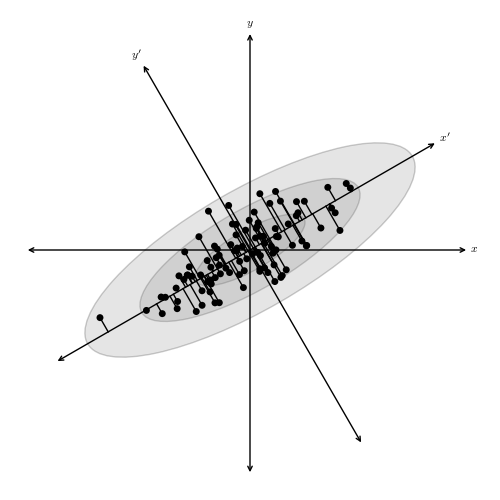
\includegraphics[width=0.37\textwidth]{fig_PCA.png}
    \caption{A distribution of points drawn from a bivariate Gaussian and centered on the origin of $x$ and $y$. PCA defines a rotation such that the new axes ($x’$ and $y’$) are aligned along the directions of maximal variance (the principal components) with zero covariance. This is equivalent to minimizing the square of the perpendicular distances between the points and the principal components}
    \label{fig:pca}
\end{figure}

\begin{remark}
	An example article, where they explain how to apply PCA on multi-wavelenght images and also mentions the pros and cons of using it.
    \begin{itemize}
    	\item Preserving Structure in Multi-wavelength Images of Extended Objects\\ \url{http://arxiv.org/abs/1101.1679v1}
    \end{itemize}
    There's a whole section that talks about this subject with a machine learning approach as a preprocessing step in this nice book,
    \begin{itemize}
    	\item Ivezi{\'c}, \v Z. and Connolly, A.J.
         and Vanderplas, J.T. and Gray, A., \textit{Statistics, Data Mining and Machine Learning in Astronomy}, Princeton University Press, Princeton, NJ, 2014.
    \end{itemize}
\end{remark}

\section{Hypothesis}\index{Hypothesis}
Our data looks like the images on Fig.\ref{fig:cubes}, and it cointains data from let's say a determined galaxy at different wavelengths, if we assume that the galaxy contains various regions that relate to interstellar objects that can tell, how stars are formed, where, how stars die, where was a star, and other mysteries, I guess we can assume that those certain regions can be identified because they share similar characteristics, the ideas is to find how a galaxy is made from, its contents, apply the concept of the superpixel idea in 3D superpixels. 
\begin{figure}[h]
	\centering
    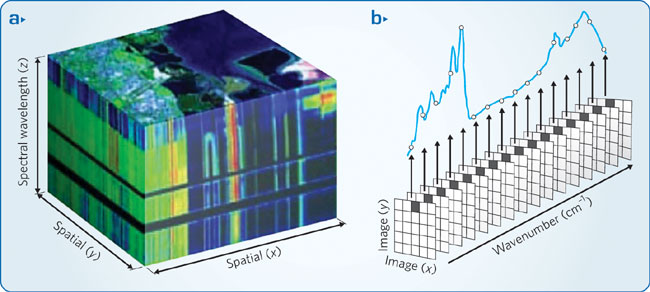
\includegraphics[width=0.57\textwidth]{nphoton.jpg}\hspace{1cm}
    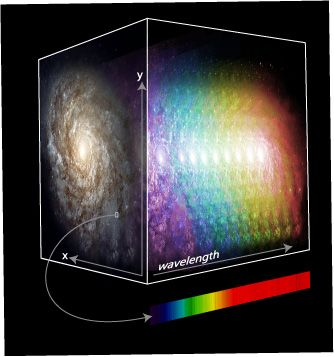
\includegraphics[width=0.27\textwidth]{data.jpg}
    \caption{Illustrations of how a datacube looks like.}
    \label{fig:cubes}
\end{figure}

Take the time to think about this, how the data looks like in 3D, how a star looks like in the datacube, imagine it, this is where ideas of how to tackle this problem come from.
\begin{figure}
	\centering
    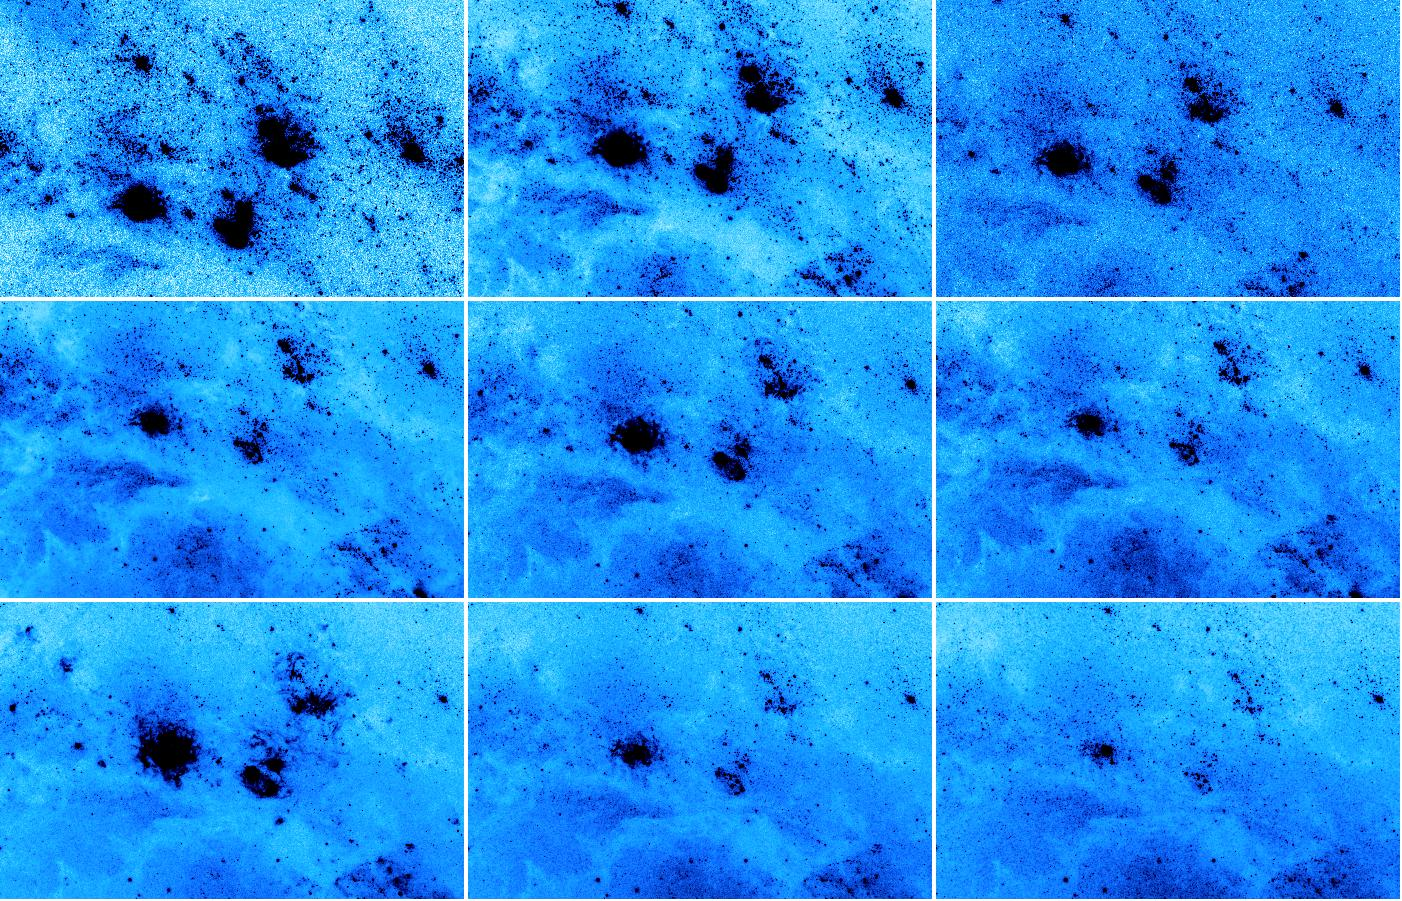
\includegraphics[width=0.87\textwidth]{nine.jpg}
    \caption{Example of how an object can look in 9 wavelenghts}
    \label{fig:nine}
\end{figure}

\subsection{Topics you should review}\index{Related topics}
This will requere a lot of work, but hey it will be worthy and fun!
\begin{itemize}
	\item Astroinformatics and computer science
    	\begin{itemize}
        	\item Data minig
            \item Machine Learning
            \item Big Data Analysis
            \item Neural Networks
            \item Visualization Resources
        \end{itemize}
    \item Statistics and Image Processing
    	\begin{itemize}
        	\item Probability Density Function
            \item Point Spread Function
            \item Full width at half maximum
            \item Convolution
        \end{itemize}
    \item Interstellar medium and star formation
    	\begin{itemize}
        	\item HII regions
            \item Planetary Nebulae
            \item Supernova Remnants
            \item Molecular Gas
            \item All kinds of Nebulae (e.g. dark, refletion)
            \item AGN's (Active Galactic Nucleus)
        \end{itemize}
    \item Astrophysics
    	\begin{itemize}
        	\item Units (light-years, parsecs)
            \item World coordinate system
        	\item Light
            \item Telescopes
            \item Stars and Stellar Evolution
            \item Distance, Brightness, Luminosity
            \item Galaxies
        \end{itemize}
\end{itemize}
The GitHub page will certainly help you to understand why you need to learn about that, and where to find articles, wepages and books.
\subsection{Downloading}
First, let's equip ourselves with the basic software you will need in order to start then you may probably find other cool programs and later you will install them. There is also the possibility that your assigned computer will have them installed already but here is a brief description of what you can do with them, most of them are easy to use.

\begin{description}
	\item[DS9:] It is a program that visualizes astronomy images in FITS format (don't worry if you recognize this format, it will be explained later), where you can easily manipulate them, read their headers, compare, look at regions, see their characteristics, make graphs, even movies. Well, depending on what you need to use later you will be finding all the functions, the best way is to click everywhere and find out what happens, also you can ask to your astronomy colleagues they will tell you all the perks, or if you like learning by yourself or you need someting specific check the documentation webpage. It is faily easy to install, just follow the instructions.
    	\begin{description}
        	\item[Download: ]\url{http://ds9.si.edu/site/Download.html}
            \item[Documentation: ]\url{http://ds9.si.edu/site/Documentation.html}
        \end{description}
        The picture below shows (Fig.\ref{fig:screen}something cool you can do in DS9.
        \begin{figure}[h]
        	\centering
    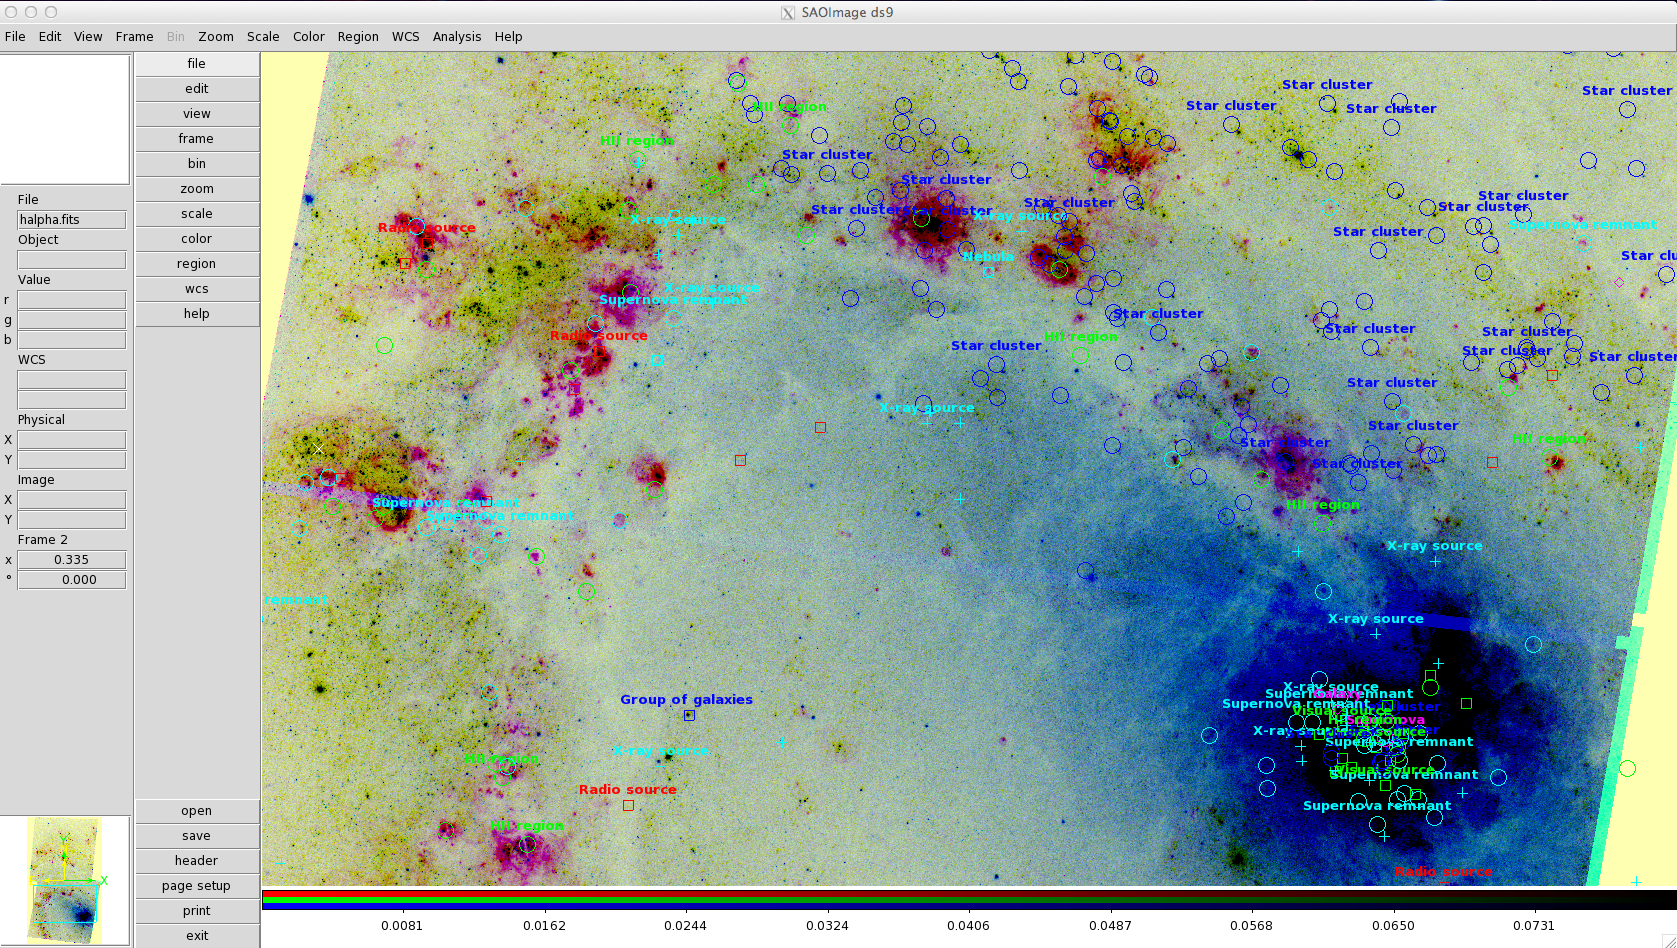
\includegraphics[width=0.87\textwidth]{Screenshot.png}
    \caption{This is an RGB picure made from 3 independent FITS files, with a zscale and a region file overlaid from NED database, if you would like to learn more about this, or reproduce it, it is all explained in this webpage: \url{https://github.com/LaurethTeX/Clustering/blob/master/NEDtoREGION-FILE/KnownRegions.md}}
    \label{fig:screen}
        \end{figure}
        
    \item[Python and a user interface: ]The most \emph{limitless} and user fiendly way to develop programs in Astronomy is using Python, there are many packages, modules, functions now available to help you in almost anything. Me, as an undergrad engineer I'm used to program on an user interface and not directly in a terminal. So, here I will explain you my own way of doing things.
    
    I make my programs on the Canopy editor, it shows when and where you have programing error and warnings, and the interface is easy to learn, now to run, I open a terminal, go to the directory where my program is, type \verb|ipython| wait and then type \verb|run| \verb|myProgram.py|, and wait for the result.
    
    Now there are a lot of fancier ways to work with \emph{Python}, you can program and test directly using \emph{IPython Notebook} on a web broswer or you can just go for the terminal, use \emph{nano} or \emph{vi} or the text editor you like and then run it by typing \verb|python| \verb|myProgram.py|. At this point is up to you, but hey here are some links to start and the packages/modules you should install.
    
    \begin{description}
    	\item[Interfaces or Development environments]\hfill
        	\begin{itemize}
            	\item PyCharm, it a development environment, just like CodeBlocks or NetBeans \url{http://www.jetbrains.com/pycharm/}
                \item Spyder, actually this is the interface that comes with the Python discritution Anaconda, you will get the Python districution and the intrerface. \url{https://store.continuum.io/cshop/anaconda/}
                \item Canopy, this is the one I mentioned before, it super easy to use and you can install packages with one click. \url{https://www.enthought.com/products/canopy/}
            \end{itemize}
        \item[Modules]\hfill
        \\
        In Python, modules are like the libraries in C, therefore, to use math, astronomy and computer science tools you need to install them. To learn whether you already have a module installed or not, type on \emph{iPython} \verb|import andreaModule|, if the output result is something like \verb|ImportError: No module named andreaModule|, you definitely don't have it installed. 
        
        The strategy here to install packages it fairly easy, find their website, go to the download section and follow the instructions, almost all the packages are available on the Python Packaing Index and may be installed by running:
        \begin{verbatim}
        	pip install pyfits
        \end{verbatim}
        To learn how to use them check the documentation page, user manuals or their API's, if you have experience on object oriented programing it will be like running a new bike and if you don't, don't worry too much, Python was designed to be easy to program, just learn the rules of the game.
        	\begin{itemize}
            	\item Astropy, this package is the \emph{must have} of every astronomer, contains tools to handle coordinate systems, units, convolution.. well is better if you take a look at the webpage. \url{http://www.astropy.org/}
                \item Numpy, this package contains the math magic functions, linear algebra tools and the array management variables, make sure you learn all about \emph{Numpy arrays} you will work with them all the time. \url{http://www.numpy.org/}
                \item SciPy, well this package is the base of all scikit modules which contain the functions you will use in image processing and machine learning. \url{http://www.scipy.org/}
                	\begin{itemize}
                    	\item Scikit Image, contains image processing tools, it is the \emph{OpenCV} for \emph{Python} \url{http://scikit-image.org/}
                        \item Scikit Learn, contains data mining algorithms, pretty much contains everything that you will ever need. \url{http://scikit-learn.org/}
                    \end{itemize}
                \item Matplotlib, this package is probably one of the most powerful tools visualize data, you can draw almost anything you want and exacly how you want it. An example of that are the images of the AstroML book, you can access to the image library code and learn how they are made, this is the website \url{http://www.astroml.org/book_figures/index.html}.\footnote{Statistics, Data Mining, and Machine Learning in Astronomy book, it was mentioned before}. You can download the package here \url{http://matplotlib.org/}.
                \item PyFITS, in this package you will find tools to manipulate FITS files, create new ones, create image cubes, tables, and do all kinds of things with their headers. Certainly this package is more than useful. \url{http://www.stsci.edu/institute/software_hardware/pyfits}
            \end{itemize}
    \end{description}
    In the path of researching I'm certain you will find more and new packages and by them you will be prepared to install anything.
    \item[Montage: ]This is a toolkit for assembling astronomical images into mosaics, but it has more functions that you may need in the future to prepare your data before processing it. There are two ways of installing and I would say that is better to have them both. One is to install the toolkit and anytime you need it, you run the commands on the terminal, the other one is to install a \emph{Python} module and use it just like any other module.
    To install montage for terminal, download the lastest version in this website \url{http://montage.ipac.caltech.edu/docs/download.html}, \textbf{read the README file} or go to this website \url{http://montage.ipac.caltech.edu/docs/build.html} and follow the steps, now if you don't have any problem installing it, you can try testing it with an example program found on this website \url{http://montage.ipac.caltech.edu/docs/pleiades_tutorial.html}, in case you are having trouble and your computer is a MAC, instead of doing step five (\emph{If you want to be able to run the Montage executables from any directory}), try this:
    
    \begin{enumerate}
    	\item Open a file called \verb|.profile| located in your user folder. (e.g. \verb|/Users/Laureth|)
        	\begin{verbatim}
            	$ vi .profile
            \end{verbatim}
         \item Include in the file the following
           \begin{verbatim}
           	export PATH=/Applications/Montage_v3.3/bin:$PATH
           \end{verbatim}
           In this link (\url{https://github.com/LaurethTeX/Clustering/blob/master/Tools.md#the-profile-file}) you will find an example of how this file should look. After you modify it, make sure that you save it and type in \verb|/Users/Laureth|,
           \begin{verbatim}
           	$ source .profile
           \end{verbatim}
           Then try testing the \emph{Montage} commands, and I'm sure that it will magically work, just remember that anytime you use any command, type \verb|source .profile|.\\
            
    \end{enumerate}
    
    
    
      Now the other way to install, implies only to install a \emph{Python} module but this module contains less functions that the terminal application, in any case check the website \url{http://www.astropy.org/montage-wrapper/}, there you will find all the documentation you may need and the instructions to install it (\emph{Spoilers} \verb|pip install montage-wrapper| ).\\
\end{description}

Any questions you may have and how to install, here is my GitHub page for software tools \url{https://github.com/LaurethTeX/Clustering/blob/master/Tools.md}

%----------------------------------------------------------------------------------------
%	CHAPTER 3
%----------------------------------------------------------------------------------------

\chapterimage{galaxy_spacewarp.jpg}
\chapter{Case Study 2:  xxxxxxxx}

Before continuing, first and most importantly you must select the \emph{raw} data you are going to process and later after you aquire experience with an specific dataset the idea is to expand the algorithms to any kind of dataset. The important things are to learn how to input the data correctly, establish the right \emph{learning paramenters} in the selected algorithm and find the best way to visualize your results and interpret them correctly.

Now let's start with basic concepts that vary from an engineering to an astronomer point of view.
\section{What is an image?}
	As you may know, an image is a matrix of numbers that cointains the specific brightness level that corresponds to a given pixel. And from there the concepts evolves and adds channels of colour and depth. But for now, let's just think about monochromatic images (only one channel). In Astronomy, images are usually considered sets of scientific data, observations, that contain information about an speficic target in the sky seen throught an specific filter and the levels of brightness correspond to the behaviour of the optical sensor (CCD camera) in relation with the number of electrons that hit a particular pixel through an specific waveband. Something else to consider is that the sky is not flat with this I mean that the celestial vault is like a sphere surrounding us therefore cartesian coorditanes are not the paramenters used to identify points in space, there is another system called WCS (World Coordinate System) hence a conversion between pixels and WCS coordinates exists. As you are realizing now just one image can contain tons of information related to it, now imagine that multiplied for terabytes and terabytes of stars, galaxies, planets, nebulae or any object in space. Fortunately in astronomy this is solved using an image format that cointains the image and its own information.
	\subsection{FITS files}
    	This format is the standard data format used in astronomy, can contain one image, multiple images, tables and header keywords providing descriptive information about the data. The way it works is that this format can contain a text file with keywords that comprise the information about the observation and a multidimensional array that could be a table, or an image, or an array of images (data cube). This files can be managed in diffetent ways, with an image preview use DS9, for handing the data in a program use the \emph{Python} package \emph{PyFITS}.
        
	\subsection{WFC3 ERS M83 Data Products}
    The selected dataset to test the data mining libraries I found is a series of observations of M83 at 9 different wavelengths, the original images can be found in this webpage, \url{http://archive.stsci.edu/prepds/wfc3ers/m83datalist.html}, the specific information about them can be found in Table \ref{tab:uno}. This particular images were observed through HST with the WFC3/UVIS camera.
    
\begin{table}[h]
  \centering
  \begin{tabular}{ c c c c c c }
    \hline\hline
    Filter / Config. & Waveband / Central $\lambda$/ Line & Obs. Date & Comment \\
    \hline
    F225W & UV filter / 235.9 nm & 26 Aug 2009 &  UV wide\\
    
    F336W & UV filter / 335.5 nm & 26 Aug 2009 & Str$\ddot{o}$mgren $u$\\
    
    F373N & Narrow-Band Filter / 373.0 nm & 19 Aug 2009 & Includes \textsc{[OII]}\\
    
    F438W & Wide-Band Filter / 432.5 nm & 26 Aug 2009 & $B$, Johnson-Cousins set\\
    
    F487N & Narrow-Band Filter / 487.1 nm & 25 Aug 2009 & Includes H$\beta$\\
    
    F502N & Narrow-Band Filter / 501.0 nm & 26 Aug 2009 & Includes \textsc{[O III]}\\
    
    F657N & Narrow-Band Filter / 656.7 nm & 25 Aug 2009 & Includes H$\alpha$+\textsc{[NII]}\\
    
    F673N & Narrow-Band Filter / 676.6 nm & 20 Aug 2009 & Includes \textsc{[SII]}\\
    
    F814W & Wide-Band Filter / 802.4 nm & 26 Aug 2009 & $I$, Johnson-Cousins set\\
    \hline
  \end{tabular}
  \caption{Summary of Observations}
  \label{tab:uno}
\end{table}
%Poner aqui la tabla con los datos de acada filtro
%No olvidar poner en GitHub el programa de como hacer el cube y tammbien el de reproject cube con montrage wrapper

\section{Preprocessing your data}
This section is where you prepare your data to be processed, you have to make sure that all your images have the same grid size, same spatial resolution, less possible quantity of outliers abd noise and same coordinate system. Now, what are those things? Same grid size means that your images must have the same pixel size, in the dataset we are processing we don't have to worry about this, the pixel size is 0.0396 arcsec/pixel. Now, spatial resoultion, each image has it's own spatial resolution depending on the filter that was used to get the observation, the number that you will be looking for is the FWHM that describes the PSF of every image. When you have all the FWHM for all the images you should choose the largest which corresponds to the poorest spatial resolution and create a convolution kernel with \emph{Tiny Tim} or use a gaussian kernel calculated with \emph{Astropy} and convolve all the images with that kernel. This exactly what I did, if you look at image \ref{img:conv}, you will see the before and after convolution. In table \ref{tab:dos} you can see how I chose the number for the FWHM.

\begin{figure}[h]
	\centering
    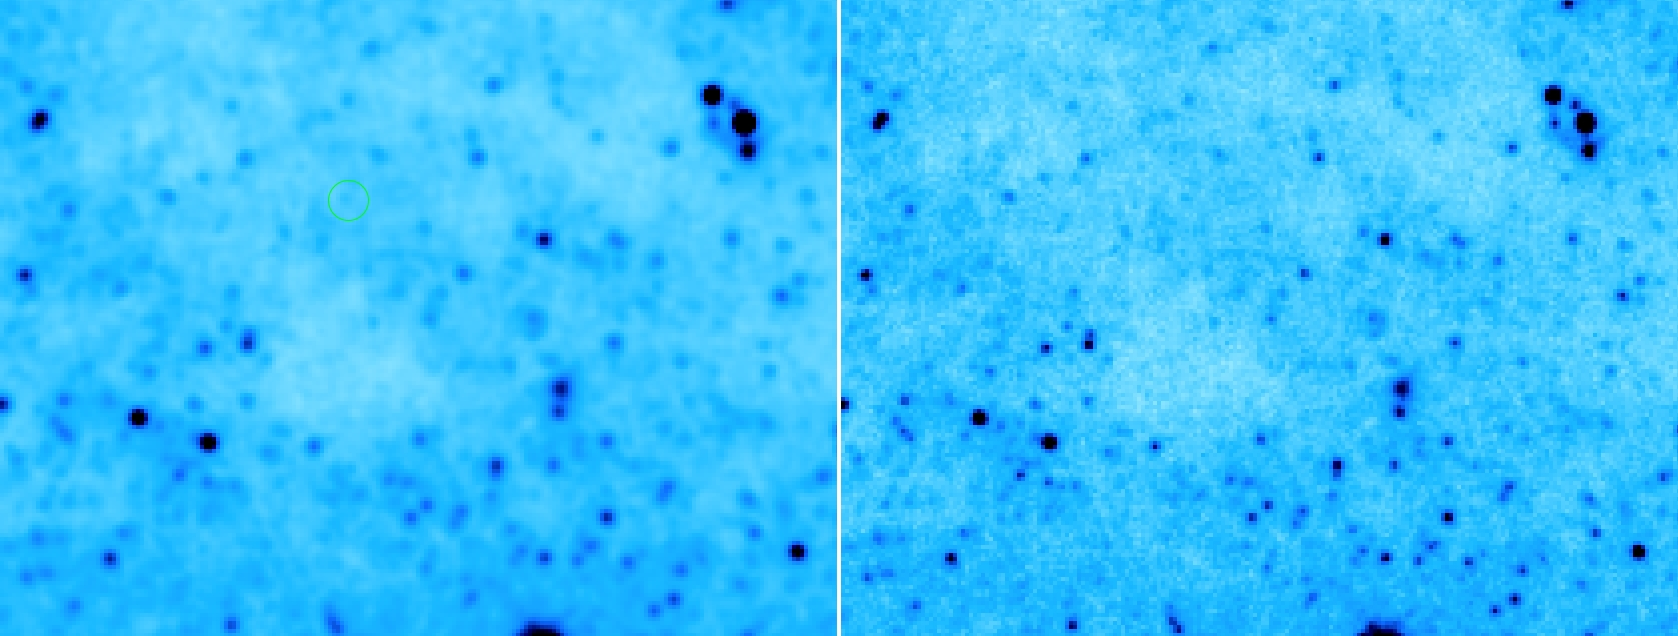
\includegraphics[width=0.87\textwidth]{conv.jpg}
    \caption{In this image you can observe how an observation looks, before and after convolution, this particular image corresponds to the B band filter and was convolved to a 0.083 arcsec FWHM}
    \label{img:conv}
\end{figure}

\begin{table}[h]
  \centering
    \begin{tabular}{ c c c }
    \hline\hline
    
    Filter / Config. & Central $\lambda$ & FWHM (arcsec)\\
    \hline
    
    F225W & 235.9 nm & $\sim$0.083\\
    
    F336W & 335.5 nm & $\sim$0.075\\
    
    F373N & 373.0 nm & $\sim$0.070\\
    
    F438W & 432.5 nm & $\sim$0.070\\
    
    F487N & 487.1 nm & $\sim$0.067\\
    
    F502N & 501.0 nm & $\sim$0.067\\
    
    F657N & 656.7 nm & $\sim$0.070\\
    
    F673N & 676.6 nm & $\sim$0.070\\
    
    F814W & 802.4 nm & $\sim$0.074\\
    
    \hline
  \end{tabular}
  \caption{WFC3/UVIS PSF FWHM informations for the selected dataset, as you can see the largest number here is 0.083 wich means the poorest spatial resolution, this is the number used to calculate the convolution kernel, in order to precess them all images must have the same spatial resolution.}
  \label{tab:dos}
\end{table}

After convoling all the picures, I started to do some tests, but I realized that maybe around 30\% of the images was missing information and/or noise and the results I was getting were mislead by the outliers. In clustering algorithms we must help the algorithm, make sure that what we are inputing is something that can be clustered, although some of them are \emph{shielded} against outliers, making our data more accesible and easy for the neural networks to interpret will help you to get better results, as you can see in image \ref{img:dos} (open one and explore it in DS9) there is missing information and noise. In order to correct this I decided to go with the easiest way I could think of, just cut the image. And I did selected a processable area excluding all the missing information and noisy areas.

\begin{figure}[h]
	\centering
    \includegraphics[width=0.47\textwidth]{uno.jpg}
    \caption{Look at the image, it is composed of two mosaics, therefore, there are some regions with missing data, now look at the borders of each mosaic there is noise near the edges, this is data that we don't want messing with our clustering algorithm and can be classifed as outliers, it is very important to reduce them as much as possbile so the output clusters can be correclty classified and correspond to the information that we are looking for}
    \label{img:dos}
\end{figure}

The next step was to build the datacube, at this point you can decide if you want to process your images indendently or all of them. The ideal here is to input all of them in a datacube, so the output cluters relate information from all the wavelenghts and the regions covered by them can be interpreted more easily. Now if you choose to create an imagecube (just append the image arrays in one FITS file) it is posible that youy images have a different conversion between their world coordinate system to pixel, so have to make sure all of your images are projected with only one conversion, this mean that you have to reproject them to a common WCS.

Well, what I wrote before it is a brief summary of what I did, but I'm sure that you can find a better way to do your own data pre-processing but here are some things that you should consider:
	\begin{itemize}
    	\item Create a methond as general as possible, with input parameter that can be adapted to any kind of data, this will save you a lot of work in the future
        \item Understand first your algorithm, how the data is going to be processed and design the best way to input your data
        \item Accomodate your data according to the type of attributes that the algorithm can handle
        \item Consider the size of your dataset, if it's huge your program may never end
        \item Find out of your algorithm can work with high dimensional data (multi-wavelenght), because if not, you won't be able to input datacubes
        \item Find out if your selected clustering algorithms is able to find clusters of irregular shapes, this will help you to device the best way to accomodate your patterns
        \item Handle outliers, if you identify them, know where they are, try to eliminate them as much as possible, we don't want them messing with our clusters
        \item In case that you come up with an artful mathematical method like PCA to reduce dimensionality, make sure that what you input can later make sense when is clustered, becuase you will be working in another space
        \item Remeber that the most important goal is to find hidden knowledge therefore, you must know you to visualize and interpret your results
        \item For the let's call it \emph{astronomy image processing}, make sure that your data is scientifically aproved ask people around you.
    \end{itemize}

%Convolution
%Cropping
%Repgojection
%Cubbing
%Explain the main rules of why to preprocess the data

This section is explained at lenght in the GitHub page, there you will find my codes and some helpful links, \url{https://github.com/LaurethTeX/Clustering/blob/master/Preprocessing.md}

\section{Software available}
%Como hacer preprocessing en los datos
For doing data preprocessing there are a bunch of softwares available, even there is one being developed by Sophia Lianou called \emph{imagecube} which, when it is finished, will be one of the best, has everything you need in one package. I'll say that this part is yours to discover, everyday there are more and more being released or new versions of the existent ones but in the meanwhile it will depend entirely on you, which software you want to use. For \emph{Python} all the functions you will need can be found in the \emph{Astropy} module, \textbf{check the API!!!.}


This specific part is all explained in GitHub in this link. \url{https://github.com/LaurethTeX/Clustering/blob/master/Preprocessing.md#first-step-data-pre-processing}

\begin{remark}
	Some links to start,
    \begin{itemize}
    	\item Astropy, Convolution and filtering, \url{http://docs.astropy.org/en/stable/convolution/index.html}
        \item AstroDrizzle: New Software for Aligning and Combining
HST Images, With Improved Handling of Astrometric Data, \url{http://drizzlepac.stsci.edu/}
		\item Tiny Tim HST PSF Modeling, \url{http://www.stsci.edu/hst/observatory/focus/TinyTim}
        \item IRAF, Image Reduction and Analysis Facility, \url{http://iraf.noao.edu/}
    \end{itemize}
\end{remark}


%----------------------------------------------------------------------------------------
%	CHAPTER 4
%----------------------------------------------------------------------------------------

\chapterimage{galaxy_spacewarp.jpg} % Chapter heading image

\chapter{Experimenting}

I discovered surfing on the internet a cloud computing software that is free, has data mining algorithms embeded, is specifically developed for Astronomy and is programmed by Caltech, University Federico II and the Astronomical Observatory of Capodimonte. The homepage website, \url{http://dame.dsf.unina.it/index.html}. Well, the platform for testing is ready!, now what? I requested and account and the next day they sent me an acceptance with my username and my password approved.
I introduced myself to the documentation, the available clustering funcionts, the manuals for every method, the blogs and discovered that the was one method available that could work with datacubes and do its clustering on every pattern (number in the multidimensional matrix) which was exaclty what I needed. The name of this method is ESOM (Evolving Self Organizing Maps) and I read its manual, did some foolish test with all my image and ... never got a result ... the experiment ran forever (more than two weeks), when I realised that this wasn't the best way to tackle this problem I started considering only clustering on the independent images and not in the datacube due to the fact that the dimensionality was inmense. So, in the end my selected methods have some results but not all, here is where all the work has to be done, analyzed and tested again.

\section{Methods Selected}

\subsection{ESOM, Evolving Self Organizing Maps}
The \emph{official} manual for this method can de found here, \url{http://dame.dsf.unina.it/documents/ESOM_UserManual_DAME-MAN-NA-0021-Rel1.2.pdf}, there you will find a full explanation of the method, the meaning of every variable and the supported file types.

Here is my own explanation of how this particular method works, first of all, can be used as an unsupervised machine learning technique or you can help the algorithm to identify regions an make it a supervised machine learnig technique, this type of clustering finds groups of patterns with similarities and preserves its topology, starts with a null network without any nodes and those are creted incrementally when a new input pattern is presented, the prototype nodes in the network compete with each other and the connections of the winner node are updated. 

The method is divided in three stages, \emph{Train}, \emph{Test} and \emph{Run}.
The first step to experiment with this method is Train. Here, the important variables to undertand an look at are, the learning rate, epsilon and the pruning frequency. It is highly recomendable that you check the DAMEWARE manual for this function, there they will explain in detail the meaning of each on the mentioned variables.
% fULL AND SAMPLE DATACUBE
\subsubsection{Expected Results}
	This particular method as I mentioned before supports datacubes and considers as an independent pattern all the  numbers in the multi-dimensional array this means that our clusters are groups of patterns with similar characteristics, that correspond to volumes of similar fluxes of electrons inside the datacube.
    
    The output files from the experiment that will show us our results are, 
    \begin{itemize}
    	\item \emph{E\_SOM\_Train\/Test\/Run\_Results.txt}: File that, for each pattern, 
reports ID, features, BMU, cluster and activation of winner node
		\item \emph{E\_SOM\_Train\/Test\/Run\_Histogram.png}: Histogram of clusters found 
        \item \emph{E\_SOM\_Train\/Test\/Run\_U\_matrix.png}: U-Matrix image 
        \item \emph{E\_SOM\_Train\/Test\/Run\_Clusters.txt}: File that, for each clusters, reports label, number of pattern assigned, percentage of association respect total number of pattern and its centroids. 
        \item \emph{E\_SOM\_Train\_Datacube\_image.zip}: Archive that includes the 
clustered images of each slice of a datacube.\footnote{I have my doubts whether this file is produced or not, in none of my test was produced, you might need to contact the developers and ask about this.}
    \end{itemize}
The file that you will be looking forward to see is the last one, the zip where you will be able to see the slices of the volume, and how the final configuration of the clusters was arranged.

\subsubsection{Failed and still running tests: What no to do and what is still running}
The first tests I did included all the complete datacube, including the areas where data was missing, the images were only reprojected and convolved. That was before realising that outliers migth affect the ability of the algorithm to identify the clusters and distract them with noise and missing data. So, the first thing you must NOT do, is to get rid of the outliers when you are training your network, if you ever get to have a well trained network then it might be interesting to learn how the network interacts with noise an outliers, but for now we will help her a bit. 

In table \ref{tab:ds9failed} are the input parameters I used to the failed tests applied in the \emph{raw} datacube, and in table \ref{tab:ds9running} are the input parameters used on experimets that are stil running since August 7th, 2014. (I wonder if they will ever end)

\begin{table}[h!]
  \centering
    \begin{tabular}{ c c c c c c }
    \hline\hline
    
    Name & Input nodes & Normalized data & Learning rate & Epsilon & Pruning Frequency\\
    \hline
    
    Train2 & 1 & 1 & 0.3 & 0.001 & 5\\
    Train3 & 1 & 1 & 0.7 & 10 & 100\\
    Train4 & 1 & 1 & 0.95 & 1 & 10\\
    Train5 & 1 & 1 & 0.99 & 0.1 & 10\\
    Train6 & 1 & 1 & 0.01 & 0.01 & 1\\
    Train7 & 1 & 1 & 0.5 & 0.7 & 5\\
    Train8 & 1 & 1 & 0.5 & 0.5 & 7\\
    Train11 & 1 & 1 & 0.25 & 0.00001 & 10\\
    
    \hline
  \end{tabular}
  \caption{This table describes all the failed experiments done in the workspace WFC3 with the \emph{raw} datacube as an input, using the ESOM method in the DAME platform selecting the number 3 as the dataset type and without using a previous configuration file.}
  \label{tab:ds9failed}
\end{table}

\begin{table}[h!]
  \centering
    \begin{tabular}{ c c c c c c }
    \hline\hline
    
    Name & Input nodes & Normalized data & Learning rate & Epsilon & Pruning Frequency\\
    \hline
    
    Train9 & 1 & 1 & 0.3 & 0.0001 & 5\\
    Train10 & 1 & 1 & 0.99 & 0.0001 & 10\\
    Train12 & 1 & 1 & 0.5 & 0.0001 & 5\\
    
    \hline
  \end{tabular}
  \caption{This table describes all the experiments done in the workspace WFC3 that are still running since August 7th, 2014 with the \emph{raw} datacube as an input, using the ESOM method in the DAME platform selecting the number 3 as the dataset type and without using a previous configuration file.}
  \label{tab:ds9running}
\end{table}

Some of the failed experiments had histogram like the one you can see on figure \ref{img:faildtrain2} where the cluters were created but reached a point where the neural network could not define how to differenciate a cluster from another clusted and failed.

\begin{figure}[h!]
	\centering
    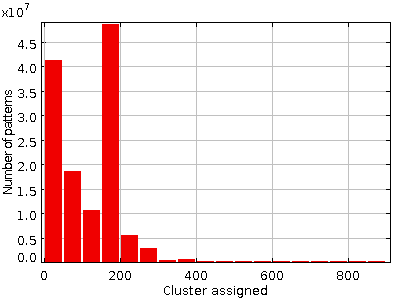
\includegraphics[width=0.47\textwidth]{Histogram_train2.png}
    \caption{In this particular experiment, the neural network failed due to a very low prunning frequency, high number of patterns and all the outliers inclusions.}
    \label{img:faildtrain2}
\end{figure}

Hey, if you were wondering why I always choose to normilize, and one as the input node, well the normalization is due to the fact that I know that the data has, according to its filter, all kinds of ranges of fluxes on every layer which means that the distances between patterns might not be correct, this is a topic you should look into. And for the input node I choose 1 because if I start with any other number the experiment automatically fails, and of course we do not want that.

As I progressed and saw the results and the \emph{log files} in all the failed experiments I decide to try the algorithm on independent layers and see if I could get something. Therefore I selected the H$\alpha$ convolved observation (halpha\_conv.fits) and did some tests on it, table \ref{tab:hafailed} shows the parameters I used for the failed experiments and table \ref{tab:harun} shows the paramters fo the still running experiments.

\begin{table}[h!]
  \centering
    \begin{tabular}{ c c c c c c }
    \hline\hline
    
    Name & Input nodes & Normalized data & Learning rate & Epsilon & Pruning Frequency\\
    \hline
    
    TrainHa1 & 1 & 1 & 0.5 & 0.01 & 5\\
    TrainHa2 & 1 & 1 & 0.5 & 0.001 & 5\\
    
    \hline
  \end{tabular}
  \caption{This table describes the failed experiments done in the workspace WFC3 for the \emph{halpha\_conv.fits} file, using the ESOM method for one layer in the DAME platform selecting the number 3 as the dataset type and without using a previous configuration file.}
  \label{tab:hafailed}
\end{table}

\begin{table}[h!]
  \centering
    \begin{tabular}{ c c c c c c }
    \hline\hline
    
    Name & Input nodes & Normalized data & Learning rate & Epsilon & Pruning Frequency\\
    \hline
    
    TrainHa3 & 1 & 1 & 0.5 & 0.0001 & 5\\
    
    \hline
  \end{tabular}
  \caption{This table describes the still running experiments since August 10th, 2014 in the workspace WFC3 for the \emph{halpha\_conv.fits} file, using the ESOM method for one layer in the DAME platform selecting the number 3 as the dataset type and without using a previous configuration file.}
  \label{tab:harun}
\end{table}

My next mental step was to repeat the tests eliminating as many outliers I could reduce, my hypothesis here is that, if I elimante all the areas where there is missing data and noise, the neural networks will be concentrated only in the patterns I'm interested in clustering and maybe idenfying interesting regions that correspond to some known interstellar object. So, what I did was to try the ESOM algorithm with, again, independent images, this time I decided to apply the same experiment to three different layers, H$\alpha$, UV wide and $i$-band. In table \ref{tab:threefail} you can see the parameters of the failed experiments and on figure \ref{img:fail3} there are some of the output histograms. Also, in table \ref{tab:threerun} you can see the input parameters of the still running experiments.

\begin{table}[h!]
  \centering
    \begin{tabular}{ c c c c c c }
    \hline\hline
    
    Name & Input nodes & Normalized data & Learning rate & Epsilon & Pruning Frequency\\
    \hline
    
    Train1 & 1 & 1 & 0.5 & 0.001 & 50\\
    Train2 & 1 & 1 & 0.5 & 0.01 & 50\\
    Train3 & 1 & 1 & 0.5 & 0.1 & 100\\
    Train4 & 1 & 1 & 0.5 & 0.001 & 100\\
    
    \hline
  \end{tabular}
  \caption{This parametes where used in three different workspaces (\emph{halphaCrop, uvwidecrop, ibandcrop}), with their own input file that corresponded to the convolved and cropped observation of each filter (halpha\_conv\_crp.fits, uvwide\_conv\_crp.fits, iband\_conv\_crp.fits), all of the experiments had no previous configuration file and the dataset type was 3 and all failed.}
  \label{tab:threefail}
\end{table}

\begin{figure}[h!]
	\centering
    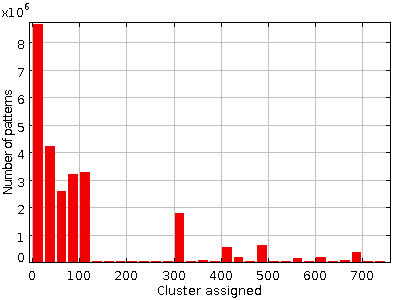
\includegraphics[width=0.31\textwidth]{Histogram-halpha1.png}
    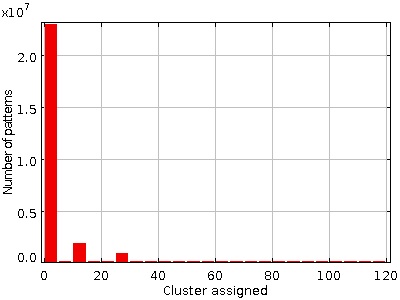
\includegraphics[width=0.31\textwidth]{Histogram-uvwide-2.png}
    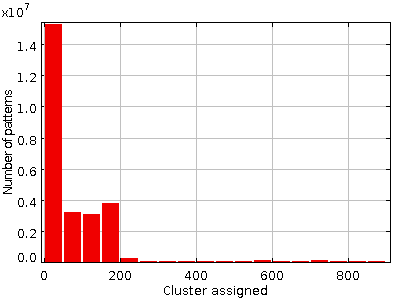
\includegraphics[width=0.31\textwidth]{Histogram-iband3.png}
    \caption{The histogram on the left corresponds to the halpha workspace in Train1, the one on the center to the iband workspace in Train3 and the one on the right to the uvwide workspace in Train2, all of them were failed experiments.}
    \label{img:fail3}
\end{figure}

\begin{table}[h!]
  \centering
    \begin{tabular}{ c c c c c c }
    \hline\hline
    
    Name & Input nodes & Normalized data & Learning rate & Epsilon & Pruning Frequency\\
    \hline
    
    Train5 & 1 & 1 & 0.5 & 0.0001 & 100\\
    Train6 & 1 & 1 & 0.99 & 0.0001 & 75\\

    \hline
  \end{tabular}
  \caption{This parametes where used in three different workspaces (\emph{halphaCrop, uvwidecrop, ibandcrop}), with their own input file that corresponded to the convolved and cropped observation of each filter (halpha\_conv\_crp.fits, uvwide\_conv\_crp.fits, iband\_conv\_crp.fits), all of the experiments had no previous configuration file and the dataset type was 3. The experiments mentioned are still running since August 11th, 2014.}
  \label{tab:threerun}
\end{table}

As you can see, I discovered that if I choose an epsilon of 0.0001 the experiments will be still running, and all of the other variables can be variated like the learning rate and the pruning frequency.

\subsubsection{The big and small reprojected datacube}
After a few days of waiting anxiously for the experiments to end and not getting any new results I decided to test the convolved, cropped and reprojected datacube including all the layers with a fixated prunning frequency of 0.0001, hopping that this time I could get some interesting results. The input parameters for the two experiments I tested can be seen in table \ref{tab:cubeesom}.

\begin{table}[h!]
  \centering
    \begin{tabular}{ c c c c c c }
    \hline\hline
    
    Name & Input nodes & Normalized data & Learning rate & Epsilon & Pruning Frequency\\
    \hline
    
    ESOMtrain1 & 1 & 1 & 0.5/0.75 & 0.0001 & 100\\
    ESOMtrain2 & 9 & 1 & 0.75 & 0.001 & 100\\

    \hline
  \end{tabular}
  \caption{This parametes where used in two different workspaces (\emph{DataCube, RPDataCube}), the first experiment is still running since August 12th, 2014 and the second failed. The input for the DataCube workspace corresponds to a 9 layer datacube with no reprojection and the RPDataCube input is the same datacube but reprojected.}
  \label{tab:cubeesom}
\end{table}

As you can see, in the experiment \emph{ESOMtrain2} I tried to start the neural network with 9 nodes (thinking logically as having 9 layers in the datacube) and immediatly the experiment failed, so \textbf{do not try to input a number different than one.}

I waited 17 days for the experiments to finish (I did some other stuff in the meanwhile, most of the time learning new things) but I did not get any results so I came up with a different strategy, selecting small datacubes with already identified regions by the NED database. I selected randomly a particular HII region located in RA 204.26971, DEC -29.84933 (See figure \ref{img:h2region}) and centered it in a 605x605 pixels sample.

\begin{figure}[h!]
	\centering
    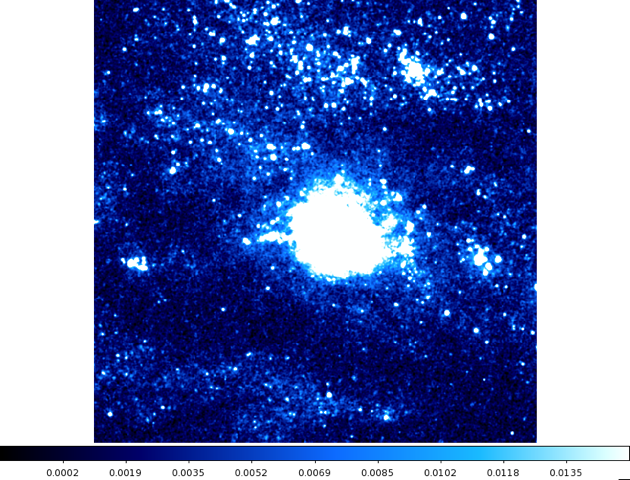
\includegraphics[width=0.52\textwidth]{small_ex.png}
    \caption{Illustration of the randomly chosen HII region for the small sample from the M83 reprojected datacube.}
    \label{img:h2region}
\end{figure}

This time, most of the experiments gave me immediate results failing or finishing. On table \ref{tab:small}, you can see the input parameters and the status of the experiments I tested with the small datacube.

\begin{table}[h!]
  \centering
    \begin{tabular}{ c c c c c c }
    \hline\hline
    
    Name & Normalized & Learning rate & Epsilon & Pruning Frequency & Status\\
    \hline
    
    ESOMtrain1 & 0 & 0.5 & 0.001 & 50 & Running\\
    Train2 & 1 & 0.5 & 0.0001 & 50 & Ended\\
    Train3 & 1 & 0.5 & 0.1 & 50 & Ended\\
    Train4 & 0 & 0.5 & 0.0001 & 50 & Running\\
    Train5 & 0 & 0.95 & 0.0001 & 100 & Running\\
    Train6 & 1 & 0.99 & 0.001 & 50 & Ended\\

    \hline
  \end{tabular}
  \caption{All the mentioned experimend belong to the SmallDataCube workspace, have 3 as data type and one input node, no previous configuration file and the input file is \emph{rp\_small\_datacube.fits}.}
  \label{tab:small}
\end{table}
In this case three of the experiments ended and none od them failed (yet), here I detected that the output file that contains the distributions of the clusters on every layer is missing, but we got some interesting resuts, in the next figures (\ref{img:smallended},\ref{img:matrixended}) you can apreciate better what I'm taking about.

\begin{figure}[h!]
	\centering
    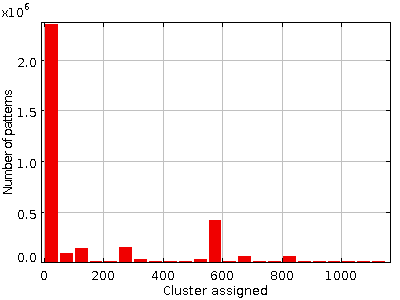
\includegraphics[width=0.31\textwidth]{Small-train2.png}
    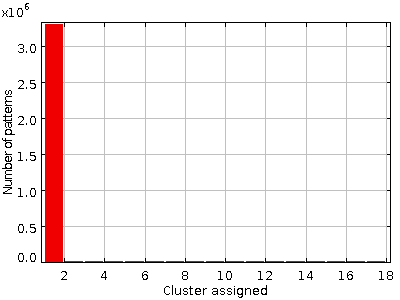
\includegraphics[width=0.31\textwidth]{Small-train3.png}
    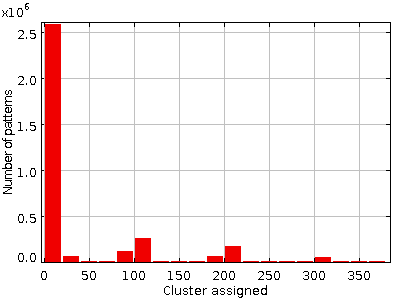
\includegraphics[width=0.31\textwidth]{Small-train6.png}
    \caption{All of the images correspond to histograms of the ended experiments mentioned above in order (Train2, Train3, Train6), as you can see there is a predominance on one of the clusters that can mean that is detecting the HII region or the experiment never started, to understand further the results a visualization of the clusters is needed.}
    \label{img:smallended}
\end{figure}

\begin{figure}[h!]
	\centering
    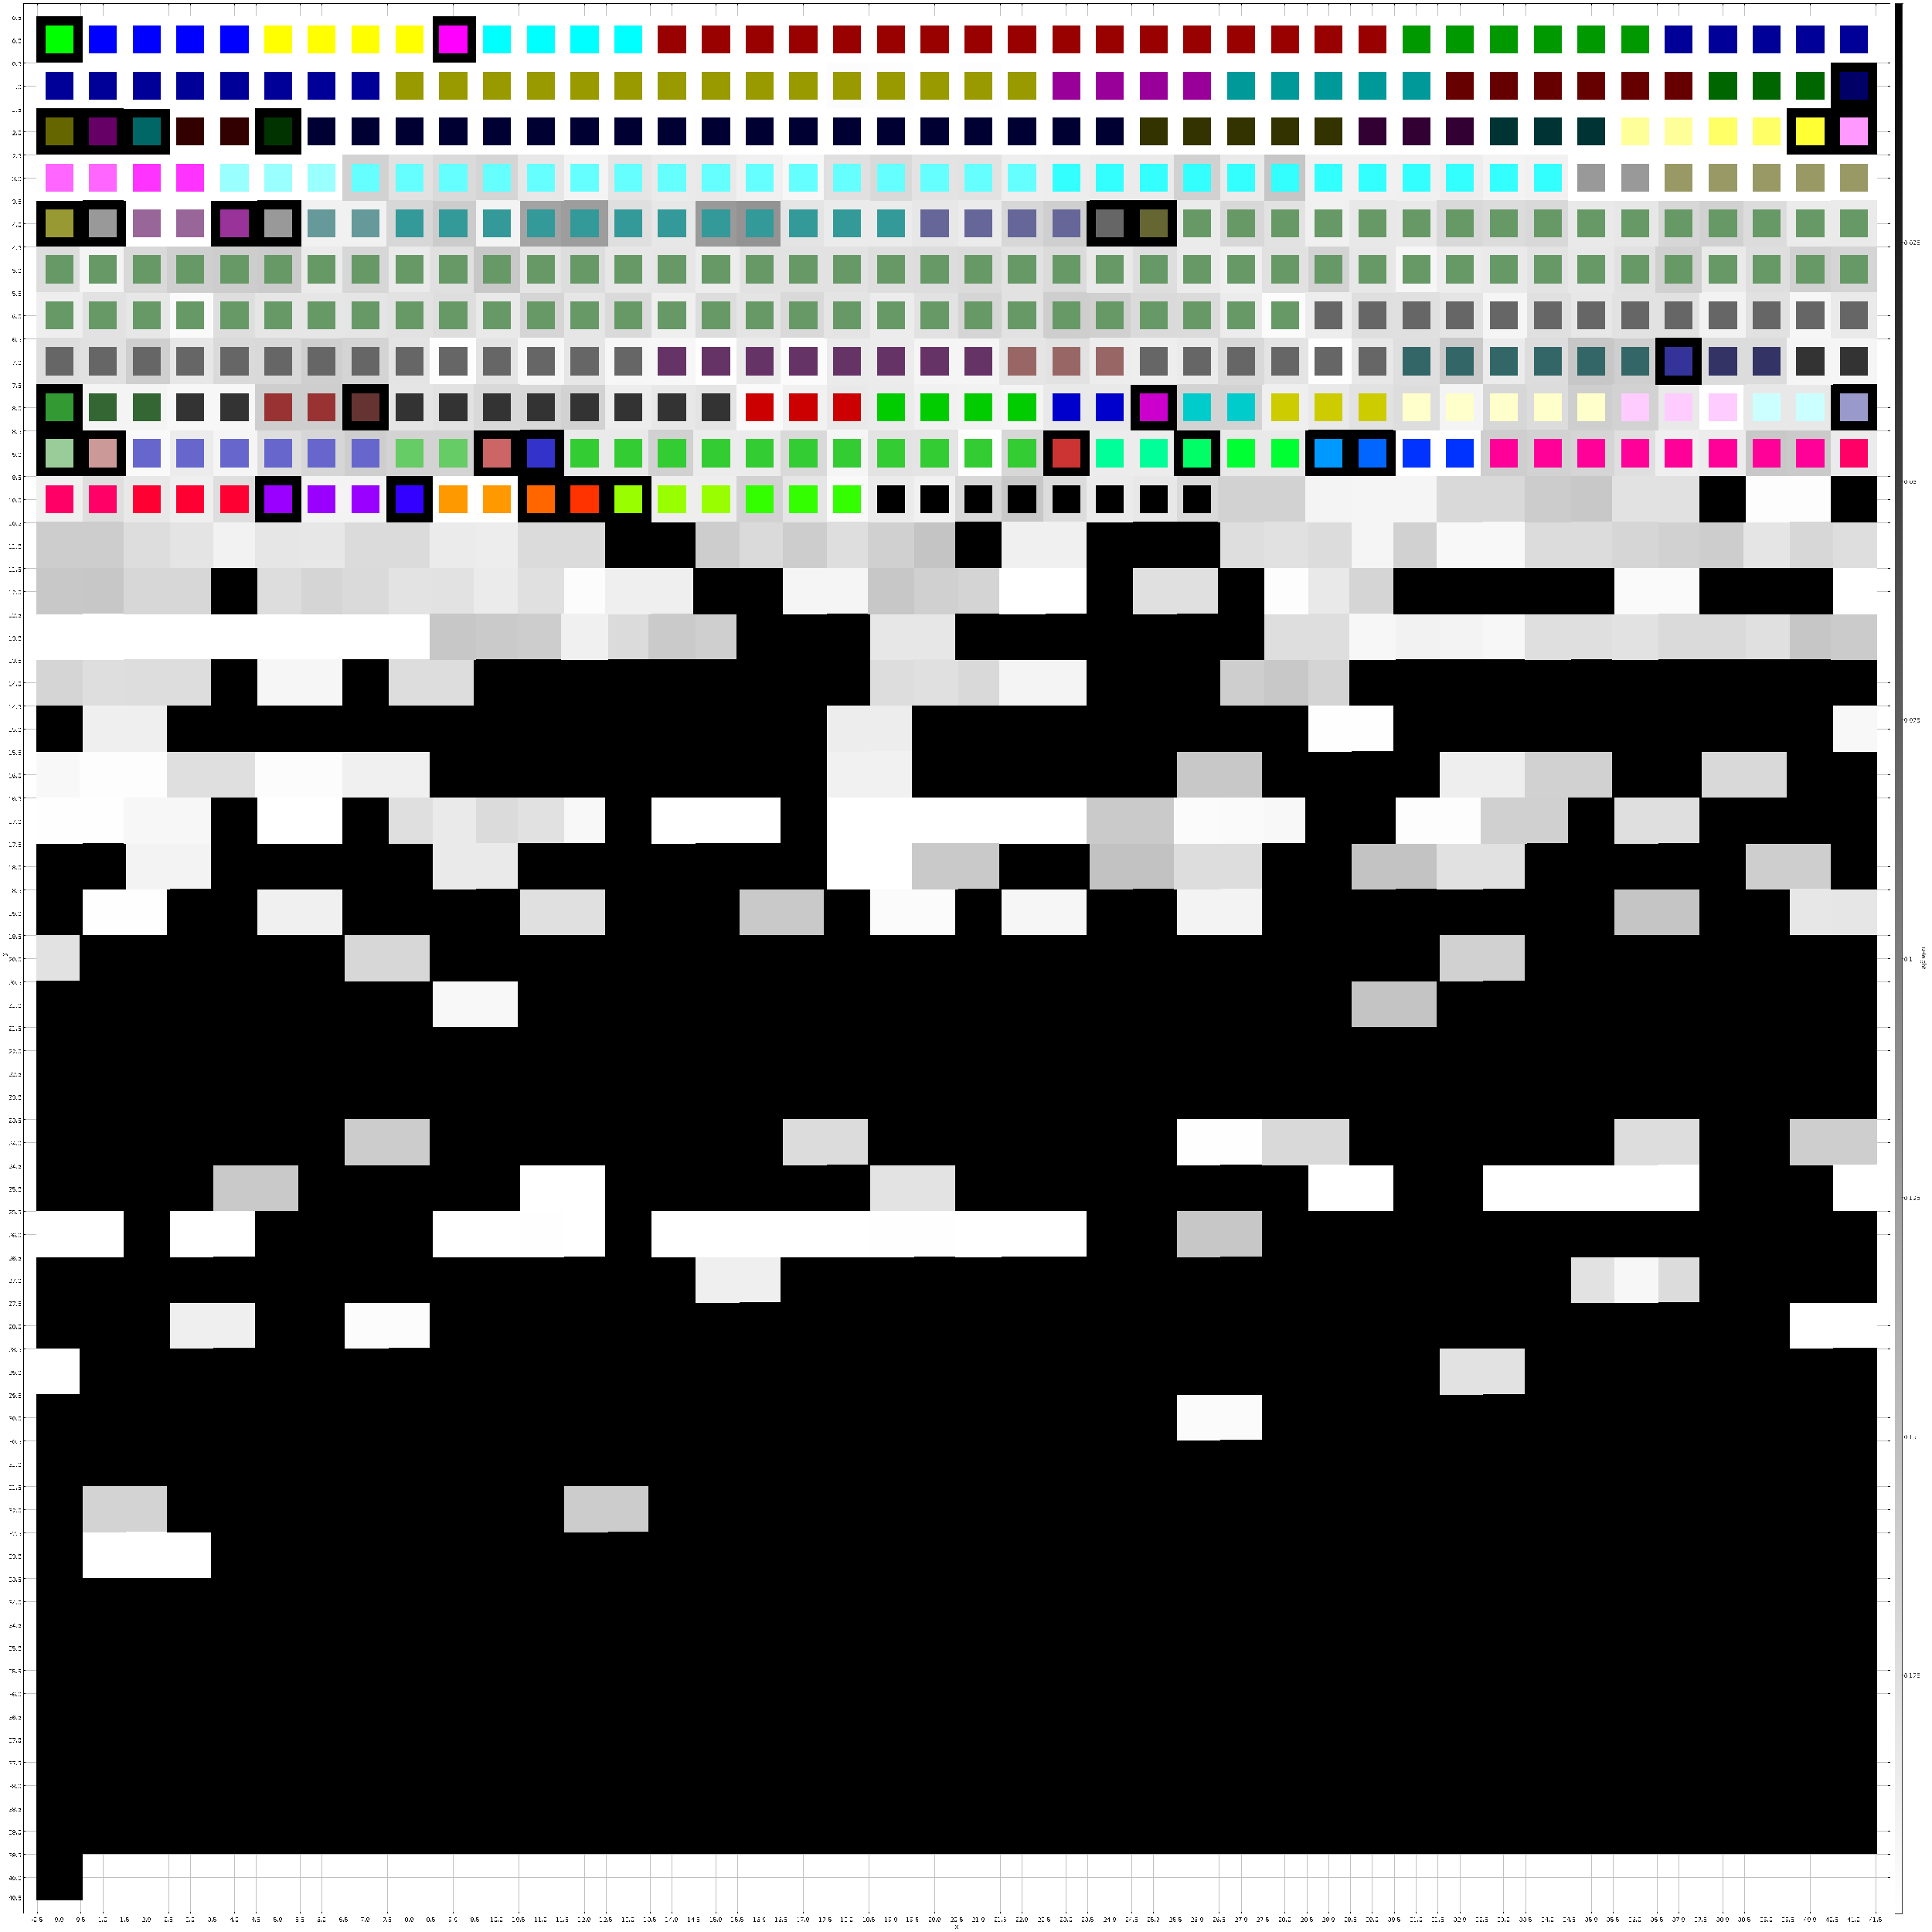
\includegraphics[width=0.31\textwidth]{matrix2-01.png}
    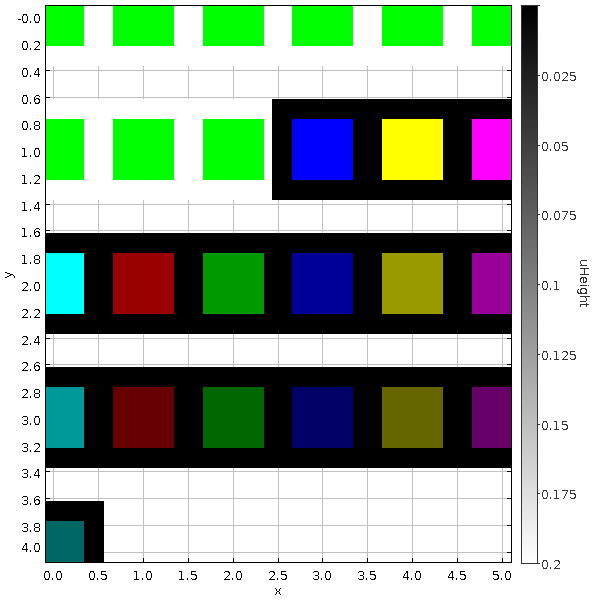
\includegraphics[width=0.31\textwidth]{Small-train3-matrix.png}
    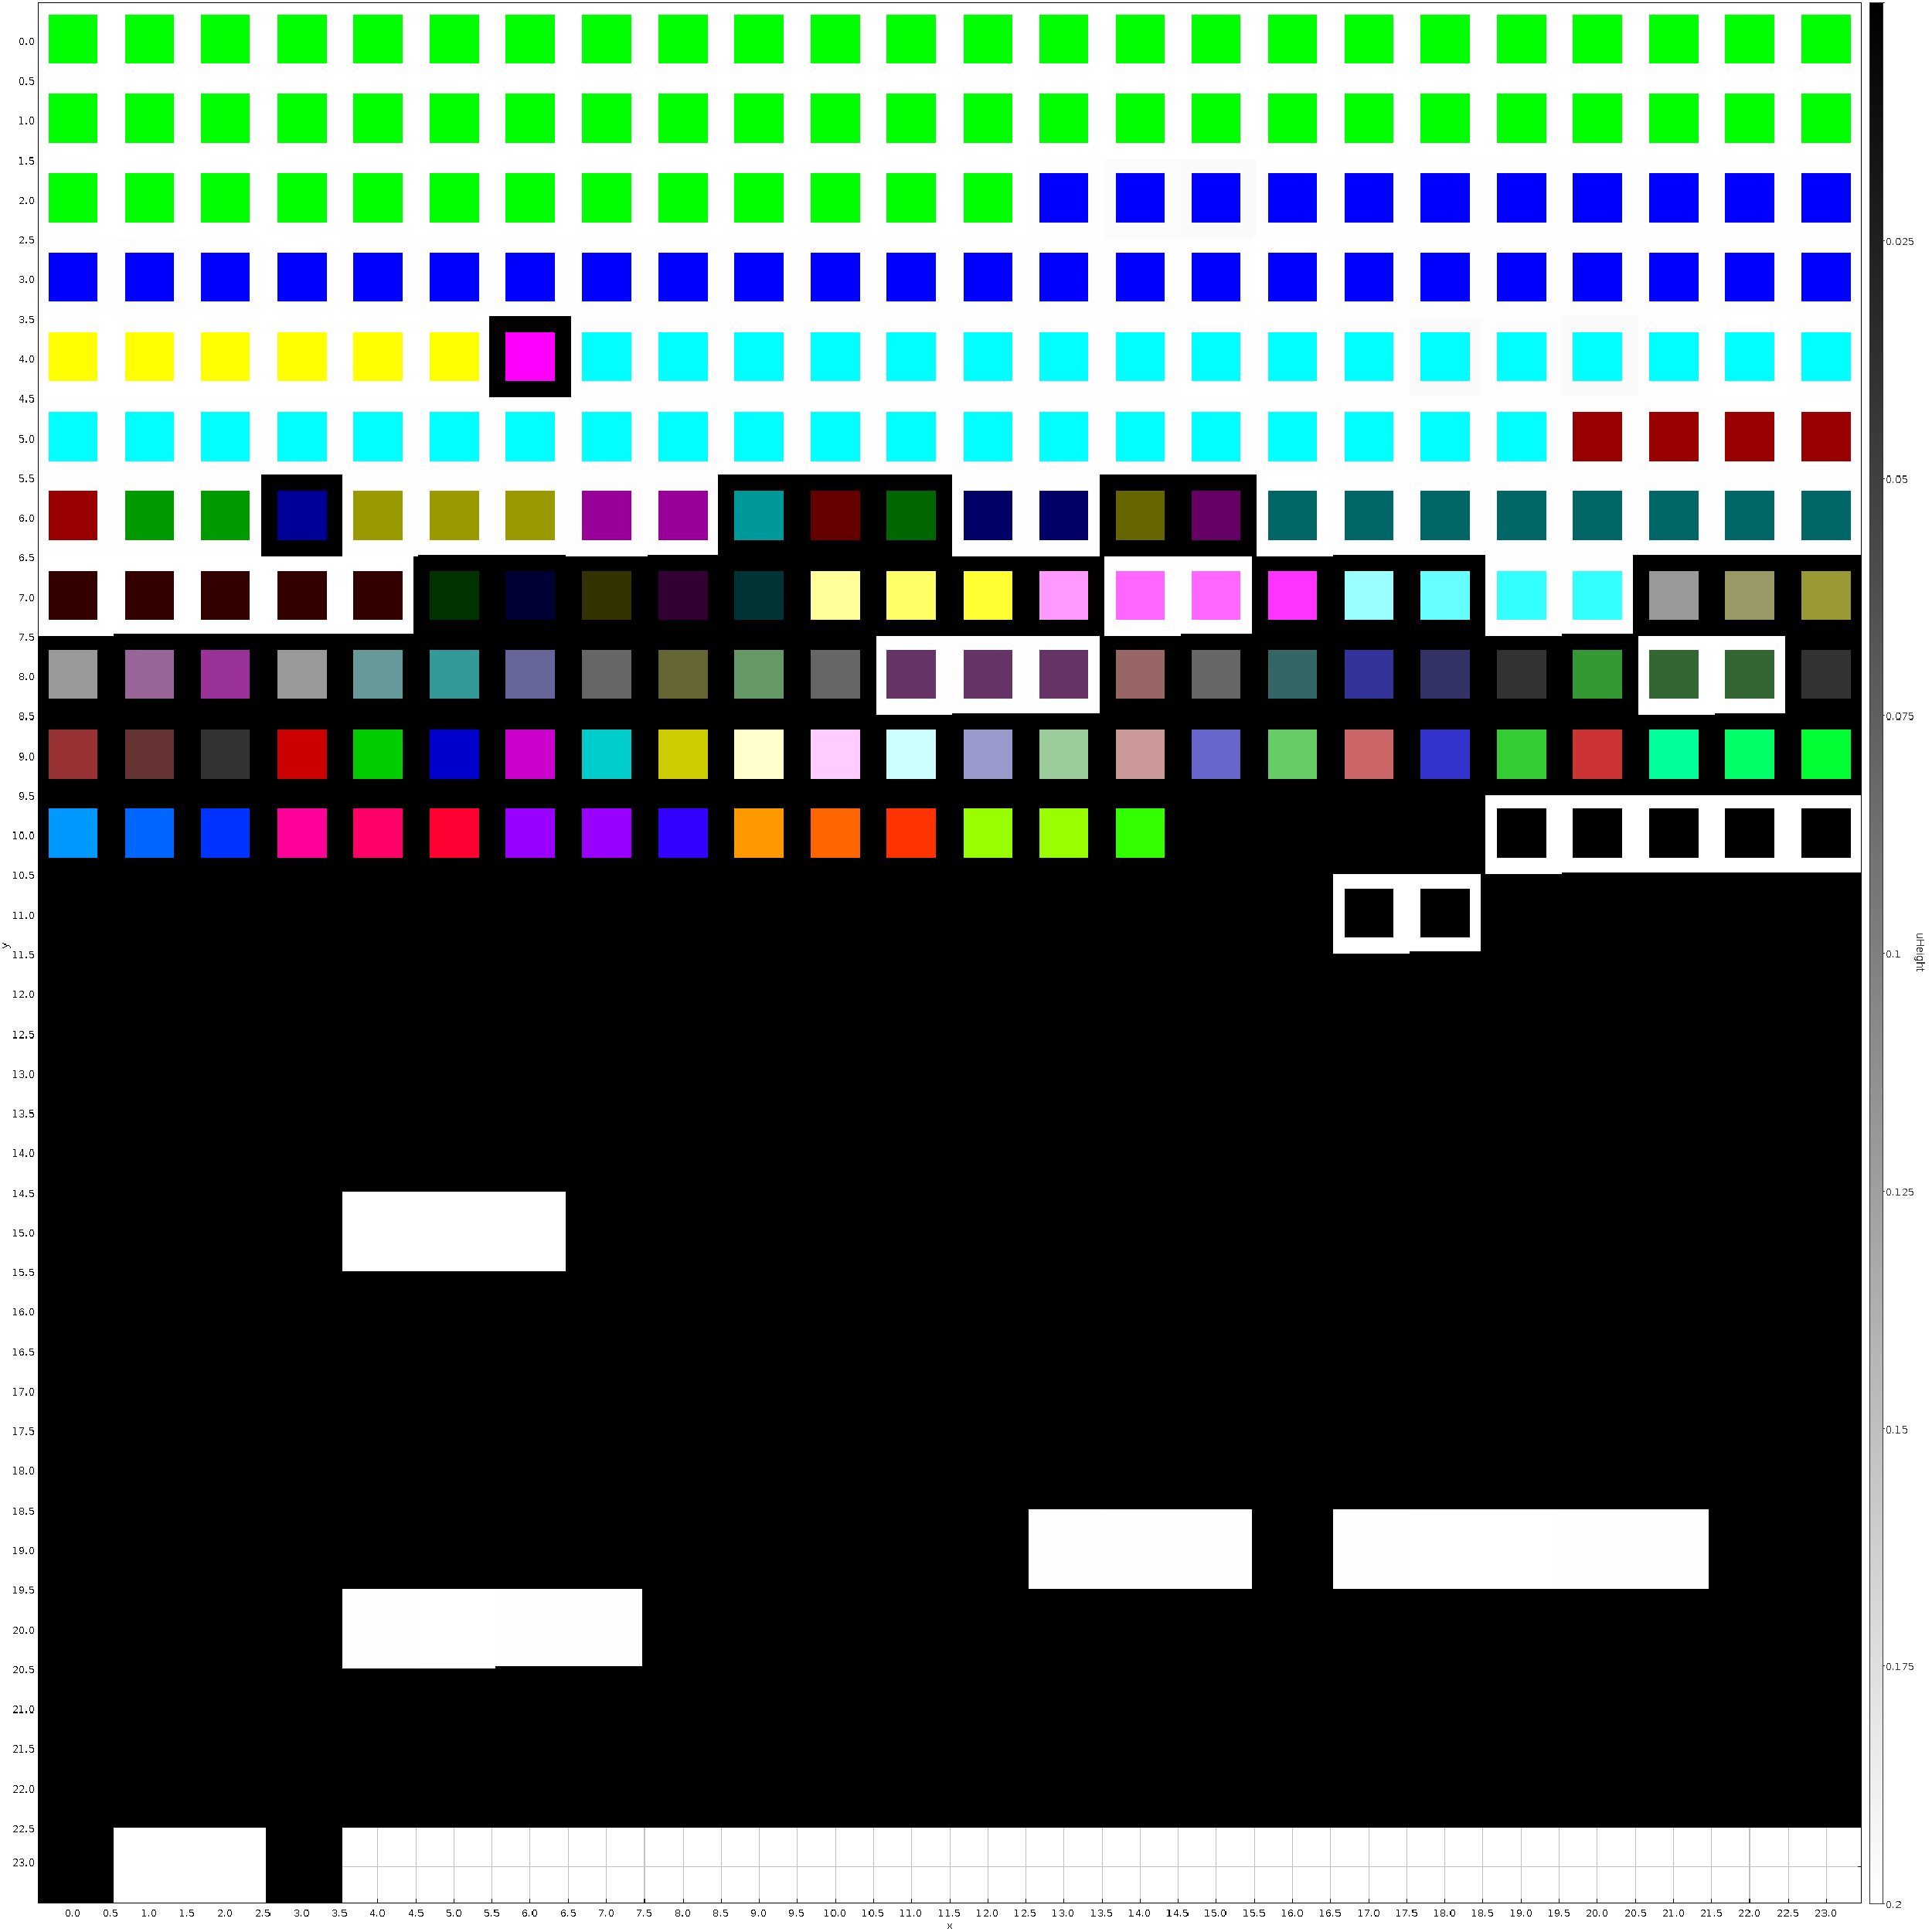
\includegraphics[width=0.31\textwidth]{matri6-01.png}
    \caption{All of the images correspond to U-matrices of the ended experiments mentioned above in order (Train2, Train3, Train6)}
    \label{img:matrixended}
\end{figure}
 There is work to be done for this cases, understand what is going on and interpret correctly the results, but last we got some.
\subsection{CSOM}
%one image
Well, as I mentioned before I did some tests using the ESOM method but since I wasn{t getting any results I thougth of testing this methond, as always I strongly recommend to read carefully its manual, \url{http://dame.dsf.unina.it/documents/SOFM_UserManual_DAME-MAN-NA-0014-Rel1.1.pdf} and fully undesrtand what is going on behind the curtains. In the meanwhile, this is my own explanation. This method uses FITS files, does not support datacubes, speciffically uses a neighborhood function in order to preserve the topological properties of the input space, it is a type of artificial network and is mainly unsupervised learning  and produces a low dimensional discretized representation of the input space of the training samples. I in this case you can choose the number of clusters/neurons in the first layer (neural network), the diameter, number of layers (in the neural network), learning rate and variance  on each layer. Here you have more input parameters to control.
\subsubsection{Expected Results}
Well in this case, since only FITS images are allowed, what we expect to find are areas indeitfying the different objects in the interstellar medium.

The important results in this case, are got in the \emph{Run} and \emph{Test} steps, in the \emph{Train} step only the network configuration is outputted. What we are interested on seein are the plotted clusters.
\subsubsection{Tests}
In this case I did some tests on the CSOM workspace, but none of the, where succesful, too many input variables to control and test. So, in this case I will leave this parameters free for you to try. I do believe that tis method could be very useful and if you find a way to input the datacube in a different configuration you will get some interesting results, due to the fact that in this method the preservation of the topology is one of the main principles.
%Mencionar los dos metodos de DAMEWARE
%Explicar los dos metodos, como untroduciste los datos, el objectivo de cada uno

%Lo que se espera obtener de cada uno de los experimentos, uno es en una sola imagen y el otro es en el datacube
%Los archivos que se obtienen y lo que significas, lo que se puede hacer



%Poner los parametros que se han elegido en los experimentos fallidos, y los que siguen en modo running
%Exlpicar por fases los experimentos que se intentaron


\section{Further work}
Well, finally we reached the point where I my time in Canada finished and I this research is still on its first stages. I have so many ideas of how to explore the clustering techniques in the DAME platform, MatLab, Python and everything else that can be tested. 

\subsection{Some interesting ideas}
%Normalizar los datos
%Acomodarlos y hacer que los paquetes sean mas pequeños
%Random points
For now, I would say that your best chance here, is to device an efficient way to input the information contained in a datacube as a list of points with values and reduce its dimensionality by randomly choosing them on every layer. If you are ever stuck, or no new ideas come to your mind, do not hesitate to contact me I might have a new interesting idea you can test.

\subsection{Links you should check out}
Most of them are listed in the useful resourses section of The Caltech-JPL Summer School on Big Data Analytics, the webpage \url{https://class.coursera.org/bigdataschool-001/wiki/Useful_resources}, you may need to create an account in Coursera and enroll in the course. And the rest of them are located in the References section on my GitHub page, \url{https://github.com/LaurethTeX/Clustering/blob/master/References.md}.
%Los links que estan en la pagina de el curso de caltech
%Sky surveys
%MATLAB SOM toolbox
%SAO datamining
\vfill
\textit{Wish you all the best, Andrea Hidalgo}
\end{document}
